\documentclass[a4paper,12pt,twoside]{memoir}

% Castellano
\usepackage[spanish,es-tabla]{babel}
\selectlanguage{spanish}
\usepackage[utf8]{inputenc}
\usepackage[T1]{fontenc}
\usepackage{lmodern} % scalable font
\usepackage{microtype}
\usepackage{placeins}

\RequirePackage{booktabs}
\RequirePackage[table]{xcolor}
\RequirePackage{xtab}
\RequirePackage{multirow}

% Añadir código python
\usepackage{listings}
\usepackage{xcolor}

% Configuración del paquete listings
\lstset{
    language=Python,                % Establece el lenguaje como Python
    basicstyle=\ttfamily\small,     % Estilo básico de fuente y tamaño
    keywordstyle=\color{blue},      % Color de las palabras clave
    commentstyle=\color{gray},      % Color de los comentarios
    %stringstyle=\color{red},        % Color de las cadenas de texto
    showstringspaces=false,         % No mostrar espacios en cadenas de texto
    tabsize=4,                      % Tamaño de la tabulación
    breaklines=true,                % Romper líneas largas automáticamente
    frame=single,                   % Agregar un marco alrededor del código
    columns=fullflexible,           % Mejorar el manejo de tabulaciones y espacios
    keepspaces=true,                % Mantener los espacios de indentación
    literate={"}{\textquotedbl}1,    % Manejar las comillas dobles correctamente
    captionpos=b                   % Caption position
}

% Links
\PassOptionsToPackage{hyphens}{url}\usepackage[colorlinks]{hyperref}
\hypersetup{
	allcolors = {red}
}

% Ecuaciones
\usepackage{amsmath}

% Rutas de fichero / paquete
\newcommand{\ruta}[1]{{\sffamily #1}}

% Párrafos
\nonzeroparskip

% Huérfanas y viudas
\widowpenalty100000
\clubpenalty100000

% Evitar solapes en el header
\nouppercaseheads


\let\tmp\oddsidemargin
\let\oddsidemargin\evensidemargin
\let\evensidemargin\tmp
\reversemarginpar



% Imagenes
\usepackage{graphicx}
\newcommand{\imagen}[2]{
	\begin{figure}[!h]
		\centering
		\includegraphics[width=0.9\textwidth]{#1}
		\caption{#2}\label{fig:#1}
	\end{figure}
	\FloatBarrier
}






\graphicspath{ {./img/} }

% Capítulos
\chapterstyle{bianchi}
\newcommand{\capitulo}[2]{
	\setcounter{chapter}{#1}
	\setcounter{section}{0}
	\setcounter{figure}{0}
	\setcounter{table}{0}
	\chapter*{#2}
	\addcontentsline{toc}{chapter}{#2}
	\markboth{#2}{#2}
}

% Apéndices
\renewcommand{\appendixname}{Apéndice}
\renewcommand*\cftappendixname{\appendixname}

\newcommand{\apendice}[1]{
	%\renewcommand{\thechapter}{A}
	\chapter{#1}
}

\renewcommand*\cftappendixname{\appendixname\ }

% Formato de portada
\makeatletter
\usepackage{xcolor}
\newcommand{\tutor}[1]{\def\@tutor{#1}}
\newcommand{\tutorb}[1]{\def\@tutorb{#1}}
\newcommand{\course}[1]{\def\@course{#1}}
\definecolor{cpardoBox}{HTML}{E6E6FF}
\def\maketitle{
  \null
  \thispagestyle{empty}
  % Cabecera ----------------
\begin{center}
  \noindent
\includegraphics[width=\textwidth]{cabeceraSalud}\vspace{1.5cm}%
\end{center}
  
  % Título proyecto y escudo salud ----------------
  \begin{center}
    \begin{minipage}[c][1.5cm][c]{.20\textwidth}
        
\includegraphics[width=\textwidth]{escudoSalud.pdf}
    \end{minipage}
  \end{center}
  
  \begin{center}
    \colorbox{cpardoBox}{%
        \begin{minipage}{.8\textwidth}
          \vspace{.5cm}\Large
          \begin{center}
          \textbf{TFG del Grado en Ingeniería de la Salud}\vspace{.6cm}\\
          \textbf{\LARGE\@title{}}
          \end{center}
          \vspace{.2cm}
        \end{minipage}
    }%
  \end{center}
  
    % Datos de alumno, curso y tutores ------------------
  \begin{center}%
  {%
    \noindent\LARGE
    Presentado por \@author{}\\ 
    en Universidad de Burgos\\
    \vspace{0.5cm}
    \noindent\Large
    \@date{}\\
    \vspace{0.5cm}
    %Tutor: \@tutor{}\\ % comenta el que no corresponda
    Tutores: \@tutor{} -- \@tutorb{}\\
  }%
  \end{center}%
  \null
  \cleardoublepage
  }
\makeatother



% Datos de portada
\title{Detección de neumonía mediante aprendizaje automático a partir de radiografías de tórax \\Documentación Técnica}
\author{Nuria Martínez Queralt}
\tutor{Daniel Urda Muñoz}
\tutorb{Natalia Busto Vázquez}
\date{\today}

\begin{document}

\maketitle



\cleardoublepage



%%%%%%%%%%%%%%%%%%%%%%%%%%%%%%%%%%%%%%%%%%%%%%%%%%%%%%%%%%%%%%%%%%%%%%%%%%%%%%%%%%%%%%%%



\frontmatter


\clearpage

% Indices
\tableofcontents

\clearpage

\listoffigures

\clearpage

\listoftables

\clearpage

\lstlistoflistings

\clearpage

\mainmatter

\appendix




\apendice{Plan de Proyecto \textit{Software}}

\section{Introducción}

En este anexo, se incluye la planificación temporal, económica y la viabilidad legal de este trabajo. La planificación temporal, engloba tanto las distintas fases del proyecto (o \textit{sprints}) como algunos de los inconvenientes que han surgido durante su desarrollo. En el caso de la planificación económica, se muestra el coste aproximado del proyecto en un periodo de 6 meses. Y, por último, en la viabilidad legal, se analizan las normativas que deben cumplirse para su correcta implementación.

\section{Planificación temporal}

Este TFG comenzó el 15 de diciembre de 2023 en una reunión con los tutores para empezar a realizar las primeras tareas, las cuales están indicadas en GitHub, en el \textit{milestone} ``Comenzar con el TFG''.

En ese momento el tema de este TFG era distinto al actual ya que, debido a diversos factores, se han tenido que realizar algunos cambios en el tema del TFG, hasta que, finalmente se ha podido realizar este.

En un principio, el tema del TFG fue ``Estadiaje de cáncer de pulmón mediante aprendizaje automático a partir de imágenes'', es decir, identificación de la existencia de cáncer de pulmón en imágenes de TAC de pacientes del HUBU empleando redes neuronales. Pero, tras una segunda tutoría, esta vez en el hospital, donde se estuvo en contacto con los médicos que iban a proporcionar dichas imágenes, se llegó a la conclusión de que no era viable trabajar con imágenes de TAC dada su complejidad. Ya que, al ser imágenes tridimensionales donde, existen múltiples cortes de la misma zona, la cantidad de datos a procesar aumenta considerablemente. Además, se debe analizar cada uno de los cortes individualmente, lo cual, representa un desafío técnico considerable. Por lo tanto, tras esta tutoría se asignó un nuevo TFG.

En este segundo TFG, la idea era emplear imágenes de CXT asociadas a un posible cáncer de pulmón de los pacientes del HUBU, las mismas imágenes que emplearía mi compañero Roberto Martínez-Guisasola Guerrero, pero, con un propósito distinto. El objetivo de este TFG era identificar cáncer de pulmón a partir de las imágenes mencionadas previamente implementando una red neuronal capaz de determinar la presencia de cáncer y señalar el lugar exacto del tumor. Esto se conseguía realizando una anotación previa de cada una de las imágenes con ayuda de un neumólogo especializado. Esta anotación consistía en, empleando un \textit{software} específico, se delimitaba en cada una de las imágenes el tumor o, en su defecto, ausencia de tumor, delimitando todo el tórax.

Pero, para comenzar a trabajar con estas imágenes era necesaria una previa aprobación por parte del comité de bioética para proteger la identidad y privacidad de los pacientes. Por lo que, tanto mi compañero Roberto como yo, tuvimos que redactar un informe al comité de bioética para presentar a fecha de 19 de febrero de 2024. Mientras se realizaba dicho informe y se esperaba a su posible aprobación o desaprobación, se realizaron otra serie de tareas indicadas en GitHub en el \textit{milestone} ``Pautas a realizar tras la tercera reunión de TFG 2/02/2024''. Entre estas tareas, cabe destacar la visualización y aplicación del video ``Real Time Face Mask Detection with Tensorflow and Python | Custom Object Detection w/ MobileNet SSD'' \footnote{\url{https://www.youtube.com/watch?v=IOI0o3Cxv9Q}} ya que, supuso bastantes problemas relacionados con el entorno de Anaconda y las versiones por lo que, se tardó mucho más tiempo del que debería. Aunque, finalmente, lo indicado en este video no fue necesario para la realización de este TFG ya que, por tercera vez se tuvo que volver a cambiar de tema.

A principios de marzo, el comité de bioética denegó la solicitud por lo que, si se quería volver a presentar, antes se tenía que realizar algún cambio. Tras considerar diversas opciones, se llegó a la conclusión de que, esperar a una posible aprobación por parte del comité de bioética suponía una pérdida de tiempo muy valioso en el desarrollo del TFG. Por lo tanto, se optó por realizar un cambio en el enfoque del TFG. 

Esta tercera y última opción consiste en, identificar una posible neumonía en imágenes de CXT obtenidas de internet implementando una red neuronal profunda. A partir de la tutoría del día 21 de marzo de 2024, se comenzó a trabajar en este TFG definitivo indicando un ``\textit{milestone}'' (o hito) por cada reunión que se ha tenido. Dentro de cada ``\textit{milestone}'' aparecen las tareas propuestas a realizar tras cada reunión.

Mencionar que, en un principio no se sabía muy bien como había que utilizar GitHub ya que, inicialmente se intentó trabajar con ZenHub, una herramienta de gestión de proyectos ágil asociada a  GitHub pero, después de mucho investigar se concluyó que, se había acabado el plazo para solicitar las plazas gratuitas para estudiantes durante un año y, ya no se disponía de acceso gratuito a esta opción por lo que, se barajaron otras herramientas como ``Asana'' o ``Jira'' pero, después de probarlas, la conclusión acabó siendo la misma y es que, había la opción gratuita durante un mes pero después, o se pagaba o las condiciones cambiaban por lo que, también se descartaron. Tras preguntar al coordinador de TFG, este indicó que, en este grado era suficiente con emplear GitHub y sus correspondientes ``\textit{milestones}'', ``\textit{issues}'' (tareas) y ``\textit{labels}'' (etiquetas). Pero, cuando llego el momento de comenzar a trabajar con GitHub y, hasta que se recordaron las nociones aprendidas en el grado y se dominó correctamente esta plataforma ya se habían realizado varias de las tareas. Por esta razón, GitHub indica un comienzo de trabajo más tardío al que realmente fue y, existen \textit{milestones} y tareas creadas y cerradas al momento (debido a que ya estaban realizadas).

Por otro lado, no se ha comenzado a trabajar con ``GitHub Desktop'' hasta empezar con el TFG definitivo y, después de algún que otro problema ya que, inicialmente no se utilizó correctamente. Por esa razón, aunque, ya se había trabajado con código de Python en el video mencionado previamente (de la segunda opción de TFG), esto no ha quedado reflejado. De todas formas, con este video se tuvo que instalar y desinstalar varias veces tanto el entorno de anaconda con el que se estaba trabajando como la aplicación de Python en sí y tampoco sirve para este TFG. Se comenzó a trabajar con código del TFG definitivo a partir de la tutoría del 21 de marzo, aunque, no se refleja en GitHub hasta principios de abril, momento en el cual, se adquirió un mayor entendimiento sobre el manejo de GitHub Desktop. Cada vez que se ha completado una tarea específica relacionada con código, se ha realizado un commit en GitHub Desktop vinculándolo con la tarea correspondiente para mantener un registro detallado del progreso y las modificaciones en el código.

También hay que tener en cuenta que, tal y como se ha indicado en GitHub, la redacción de la memoria se comenzó previamente a crear el \textit{milestone} ``Redacción de la memoria'' ya que, dentro de otros \textit{milestones} asociados a cada reunión ya existen tareas relacionadas con la redacción de la memoria. 

El \textit{milestone} de ``Lecturas bibliográficas neumonía'' y ``Lecturas bibliográficas neumonía con \textit{deep learning}'' hacen referencia a la lectura de los artículos para la posterior redacción del estado del arte acorde a esos artículos. Lo mismo sucede con el \textit{milestone} ``Lecturas bibliográficas redes neuronales'', el cual se refiere a la lectura del libro para adquirir conocimientos y aportar información en diversas secciones de la memoria, sobre todo en el apartado de ``\textit{Conceptos teóricos}''.

La fecha de vencimiento indicada en algunos \textit{milestones} de las reuniones, se refiere a una fecha orientativa para la realización de las tareas indicadas, generalmente dos semanas, pero, aunque se hubieran realizado todas las tareas, el cerramiento de las ``\textit{issues}'' y ``\textit{milestones}'' no se llevaba a cabo hasta la siguiente tutoría por si quedaba alguna duda relacionada con esas tareas o algo no estaba completo.

Tras esta extensa explicación de la planificación indicada en GitHub y todos los problemas que han surgido, se puede decir que la planificación seguida ha sido la siguiente:

\textbf{\textit{Sprint} 1: ``Comenzar con el TFG'' del 15/12/23 al 24/1/24} 
\begin{itemize}
    \item Descargar y empezar a trabajar con la plantilla de LaTex
    \item Visualización del video colgado en ubuvirtual acerca de los distintos puntos a tener en cuenta en el TFG
    \item Crear repositorio en GitHub
    \item Empezar a trabajar con keras y MNIST desde Python
    \item Hacer una primera revisión para buscar información del cáncer de pulmón en artículos, en la OMS, etc.
    \item Rellenar la solicitud para el acceso a SCAYLE
\end{itemize}

\textbf{Nota 1:} Este \textit{sprint} tiene una duración de más de un mes debido a que coincidió con todos los exámenes finales del primer semestre.

\textbf{Nota 2:} la tarea de ``Crear repositorio en GitHub'', lleva consigo algunos problemas mencionados previamente y por eso, este primer \textit{sprint} no se creó hasta el 18 de febrero en GitHub

\textbf{\textit{Sprint} 2: ``Redefinición TFG'' del 29/1/24 al 18/2/24}
\begin{itemize}
    \item Realización del informe de solicitud para el comité de bioética 
\end{itemize}

\textbf{\textit{Sprint} 3: ``Pautas a realizar tras la tercera reunión de TFG 2/02/2024'' del 2/2/24 al 13/3/24}
\begin{itemize}
    \item Visualización del video ``Real Time Face Mask Detection with Tensorflow and Python | Custom Object Detection w/ MobileNet SSD'' \footnote{\url{https://www.youtube.com/watch?v=IOI0o3Cxv9Q}} para realizarlo en un script de Python
    \item Crear un nuevo entorno virtual en anaconda para trabajar en el TFG
    \item Investigar como trabajar con la plantilla de overleaf (LaTex)
    \item Comenzar a leer el libro ``Fundamentos de visión por computador'' para entender mejor algunos conceptos importantes para este trabajo y para servir de ayuda en la redacción de la memoria
\end{itemize}

\textbf{Nota 1:} Este \textit{sprint} se solapa con el anterior debido a que, el anterior pertenece a la tutoría realizada en el hospital donde se indicó esa tarea a realizar y, se acordó una nueva tutoría para poder avanzar con otras tareas a la vez que se realizaba el informe.

\textbf{Nota 2:} Como ya se ha comentado previamente, la visualización de este video, supuso una serie de problemas por lo que, en este periodo de tiempo se solicitaron varias tutorías para solucionar cada uno de los problemas que iban surgiendo pero, no se indicaban nuevas tareas y, por tanto no se visualizan como nuevos \textit{sprints}.

\textbf{\textit{Sprint} 4: ``Reunión 13/3/24'' del 13/3/2024 al 21/3/24}
\begin{itemize}
    \item Comenzar a trabajar con GitHub Desktop
\end{itemize}

\textbf{Nota 1:} Esta reunión no está reflejada en GitHub debido a que fue en medio de todo el proceso de cambio de TFG dónde no se sabía cuál iba a ser el TFG definitivo y, por lo tanto no habían tareas claras a realizar hasta que esto no se decidiera. Además, aunque a partir de esta reunión se comenzó a trabajar con GitHub Desktop, no fue hasta un par de tutorías más tarde que, se empezó a trabajar de la forma correcta con esta herramienta. 

\textbf{Nota 2:} A partir del siguiente \textit{Sprint} ya se empieza a trabajar con el TFG definitivo

\textbf{\textit{Sprint} 5: ``Primera reunión con el TFG definitivo 21/03/2024'' del 21/3/24 al 8/4/24}
\begin{itemize}
    \item Modificar el código de MNIST sacado de internet para acceder a imágenes ya descargadas en lugar de imágenes de internet.
    \item Modificar el código de MNIST sacado de internet para un problema de clasificación binaria
    \item Comprobar que el código funciona correctamente entrenando 10 épocas y calcular una serie de métricas como \textit{accuracy}, sensibilidad, sensitividad, AC o F1.
\end{itemize}

\textbf{\textit{Sprint} 6: ``Reunión TFG 8/4/24'' del 8/4/24 al 3/5/24}
\begin{itemize}
    \item Investigar acerca del parámetro callback (\textit{Early Stopping}) y añadirlo en la parte de conceptos teóricos de la memoria
    \item Modificar parámetros de la función model.fit (para entrenar el modelo), añadiendo el callabck (\textit{Early Stopping})
    \item Realización de métricas a mano en lugar de, automáticamente con keras
    \item Crear distintos modelos con distintas arquitecturas (Simple1, Simple2...), variando el número de neuronas/capas para comparar los resultados con un determinado \textit{batch size}.
    \item Investigar acerca del valor de \textit{batch size} en \textit{train} y como este afecta en el resultado y añadirlo en la parte de conceptos teóricos de la memoria
    \item Probar distintos valores de \textit{batch size} para las distintas arquitecturas realizadas previamente
    \item Comparación de las distintas arquitecturas para distintos \textit{batch size} y escoger la mejor opción en cuanto a métricas
    \item Realización en Python (u otro programa) de tablas y/o gráficas para visualizar los resultados de las métricas para las distintas arquitecturas en distintos \textit{batch size}
    \item Comenzar con la lectura de los artículos indicados en el milestrone ``Lecturas bibliográficas neumonía'' para la redacción del estado del arte de la memoria
    \item Comenzar a redactar tanto el resumen como la introducción 
\end{itemize}

\textbf{Nota:} La redacción del resumen y la introducción, no está indicada en el \textit{milestone}  porque, en un principio no era una tarea de este \textit{sprint} pero, una vez se empezó a redactar en la memoria, se decidió comenzar con estos dos puntos.

\textbf{\textit{Sprint} 7: ``Reunión TFG 3/5/24'' del 3/5/24 al 16/5/24}
\begin{itemize}
    \item Volver a intentar la realización de todas las métricas a mano ya que en el \textit{sprint} anterior solo se acabaron consiguiendo unas pocas.
    \item Modificación del código realizado previamente para adaptarlo a estas nuevas métricas
    \item Analizar los resultados obtenidos. Redactar en la memoria la comparativa de las tablas/gráficas y el porqué de los resultados obtenidos.
    \item Explicar en la parte de ``metodología'' de la memoria cómo se va a trabajar con las diferentes tablas (en este caso \textit{batch size} y \textit{EarlyStopping})
    \item Una vez elegida la mejor arquitectura y el mejor \textit{batch size}, se prueban distintos valores de neuronas (32, 64, 128, 156) para la capa o capas ocultas y se selecciona la mejor opción.
    \item Analizar en el apartado de ``Resultados'' de la memoria, los resultados obtenidos con distintos valores de neuronas
    \item Explicar en la parte de ``Metodología'' de la memoria cómo se va a trabajar con la tabla donde se compara el número de neuronas.
    \item Redactar en el apartado de ``Conceptos teóricos'' información acerca de redes neuronales, aprendizaje automático y aprendizaje profundo.
    \item Redacción del estado del arte a partir de los artículos del \textit{milestone} ``Lecturas bibliográficas neumonía'' y ``Lecturas bibliográficas neumonía con \textit{deep learning}''
    \item Avanzar en otros puntos de la memoria como conceptos teóricos y objetivos
\end{itemize}

\textbf{\textit{Sprint} 8: ``Reunión TFG 16/5/24'' del 16/5/24 al 24/5/24}
\begin{itemize}
    \item Comenzar a redactar el anexo de planificación e incluir en el apartado de ``\textit{Aspectos relevantes}'' de las conclusiones, todos los inconvenientes que han surgido durante la realización de este trabajo
    \item Modificación de la bibliografía para solucionar algunos errores
    \item Modificar el número de épocas a 20 en las tablas realizadas previamente para poder observar mejores resultados
    \item Modificar las tablas realizadas previamente eliminando el índice, y redondeando los decimales de la tabla a 2 para que se puedan visualizar mejor los resultados en el documento.
    \item Tras cambiar el número de épocas, puede que los resultados cambien, por lo tanto, si esto sucede, se deben modificar los resultados en la memoria.
    \item Revisar y dejar correctamente escrito toda la parte de introducción, resumen, conceptos teóricos escritos hasta ahora, estado del arte, parte de la metodología redactada hasta ahora y parte de los resultados redactados hasta ahora.
\end{itemize}

\textbf{\textit{Sprint} 9: ``Reunión TFG 24/5/24'' del 24/5/24 al 3/6/24}
\begin{itemize}
    \item Realización de una función para dividir el número de imágenes de forma correcta ya que, tal y como están distribuidas las imágenes en el dataset original se complica la obtención de buenos resultados.
    \item Redactar en el apartado de ``\textit{Descripción de los datos}'' la nueva división de imágenes.
    \item Modificar parámetros y averiguar por qué no se obtienen buenos resultados en las tablas comparativas realizadas previamente
\end{itemize}

\textbf{\textit{Sprint} 10: ``Reunión TFG 3/6/24'' del 3/6/24 al 17/6/24}
\begin{itemize}
    \item Modificación y ejecución de código para ver si los resultados de las tablas mejoran ya que, los resultados obtenidos continúan siendo malos sin explicación alguna. Esto incluye la creación de la CNN AlexNet para hacer las correspondientes comparaciones.
    \item Creación de gráficas para visualizar el rendimiento del modelo en el entrenamiento y la validación y explicar estos resultados en la memoria
    \item Realizar modificaciones en la memoria y anexos (sobre todo en la parte más biológica) acorde al feedback recibido tras el envío del primer borrador de la memoria.
    \item Completar toda la información tanto en la memoria como en los anexos para poder enviar el primer borrador completo del TFG a ambos tutores.
    
    

\end{itemize}

\textbf{\textit{Sprint} 11: ``Reunión TFG 17/6/24'' del 17/6/24 al 28/6/24}
\begin{itemize}
    \item Para que se guarden los modelos que se ejecutan tras cada entrenamiento y, así poderse reutilizarlos en caso necesario (como para la creación de la matriz de confusión), se ha de añadir ``model.save'' y, después ``model.load'' para recuperar el modelo
    \item Modificar memoria y anexos acorde a los nuevos resultado
    \item Completar el apartado ``Pruebas del sistema'' dentro del anexo manual del programador
    \item Crear una carpeta ``resultados'' con python donde se encuentren todos los csv de los históricos para que estén más ordenados
    \item Añadir todas las carpetas/documentos empleados en este trabajo en el repositorio de GitHub
    \item Ejecutar notebook del archivo.py
    \item Rematar todos los anexos y memoria para poder entregar un borrador a los tutores
\end{itemize}

Para concluir, en la figura \ref{fig:grafica_planificacion} se muestra gráficamente el ritmo de trabajo llevado a cabo durante este proyecto. En esta gráfica, se pueden observar dos picos significativos en la actividad, uno al inicio y otro al final. Y es que, tal y como se ha comentado previamente, GitHub se comenzó a usar posteriormente al comienzo del proyecto por lo que, todas las tareas que ya se habían realizado previamente se tuvieron que abrir y cerrar al momento. Por otro lado, el pico final, se corresponde con la redacción y revisión final de cada uno de los apartados de la memoria y los anexos. Y, dado que estas revisiones se estuvieron realizando hasta el último momento, las tareas se han cerrado de forma simultánea al finalizar el proyecto.

\begin{figure}[h]
        \centering
        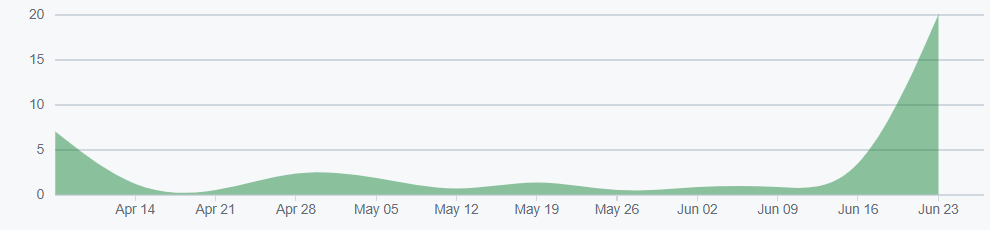
\includegraphics[width=0.99\textwidth]{img/grafica_planificacion.PNG}
        \caption{Contribución de las tareas realizadas con GitHub. Fuente propia.}
        \label{fig:grafica_planificacion}
    \end{figure}

\subsection{Planificación económica}

Los costes se van a calcular sobre un periodo aproximado de 6 meses tanto a nivel de personal como de \textit{hardware} y de \textit{software}.

\subsubsection{Personal}

Aunque el salario de un ingeniero es mayor que el salario mínimo mensual, en este caso se va a calcular la planificación económica a nivel de personal con esa referencia para conseguir un coste aproximado. Tabla \ref{tab:personal}.

El salario mínimo mensual neto en 2024 es de 1.134 euros en 14 pagas o 1.323 euros mensuales en 12 pagas ~\cite{grupo200024}. A esto hay que sumarle el IRPF y la seguridad social. Respecto al IRPF en 2023 era del 19\% pero, tras la subida de sueldo en 2024, el gobierno aprobó una rebaja del IRPF para el salario mínimo por lo que, al tratarse de un sueldo de 15.876 euros anuales no habría retención del IRPF ~\cite{MinHa24} (esto cambiaría en caso de que el sueldo fuera mayor). El porcentaje de salario destinado a la seguridad social es del 28,3\% ~\cite{GoEs24}.

\begin{table}[h]
    \centering
    \begin{tabular}{cc}
        
        Salario mínimo mensual & 1.134 euros \\ 
        \toprule
         IRPF (0\%) & 0 euros \\ 
         \toprule
         Seguridad social (28,3\%) & 320,92 euros \\ 
         \toprule
         Salario mensual bruto & 1454,92 euros \\ 
         \toprule
         \textbf{Total en 6 meses} & \textbf{8729,53 euros} \\ 
         
    \end{tabular}
    \caption{Costes de personal}
    \label{tab:personal}
\end{table}

\subsubsection{\textit{Hardware}}

Para calcular los gastos del \textit{hardware}, se va a calcular el gasto aproximado que supone el ordenador en 6 meses partiendo del precio original del ordenador empleado y teniendo en cuenta que se tiene desde hace tres años y medio aproximadamente. Tabla \ref{tab:hardware}.

\begin{table}[h]
    \centering
    \begin{tabular}{ccc}
        \toprule
        \textbf{Concepto} & \textbf{Costes} & \textbf{Amortización 6 meses}\\
        \toprule
        Portátil ``Lg Gram'' & 1400 euros (aprox) & 200 euros (aprox)\\
    \end{tabular}
    \caption{Costes de \textit{hardware}}
    \label{tab:hardware}
\end{table}

\subsubsection{\textit{Software}}

En cuando al \textit{software}, todos son de código abierto y su uso es gratuito.

\subsubsection{Coste total}

En la tabla \ref{tab:total} se muestra el coste total aproximado que supone este proyecto en un periodo de 6 meses. 

\begin{table}[h]
    \centering
    \begin{tabular}{cc}
        Personal & 8729,53 euros \\
        \toprule
        \textit{Hardware} & 200 euros\\
        \toprule
        \textit{Software} & 0 euros \\
        \toprule
         \textbf{Total} & \textbf{8929,53 euros} \\
    \end{tabular}
    \caption{Coste total}
    \label{tab:total}
\end{table}

\subsection{Viabilidad legal}

Tal y como se ha indicado en el \textit{Anexo A}, se han comenzado diversos planteamientos de TFG antes de llegar al definitivo. En la segunda propuesta, en la cual se iban a emplear imágenes de pacientes del HUBU, fue necesaria la realización de un informe del comité de bioética para poder trabajar con dichas imágenes asegurando que en ningún momento se conoce la identidad del pacientes ya que las imágenes están anonimizadas siguiendo la \textbf{Ley Orgánica de Protección de Datos y Garantía de Derechos Digitales (3/2018)}. 

Pero, como ya se ha comentado también en el \textit{Anexo A}, esta solicitud fue denegada en un primer momento y, por lo tanto, se ha acabado trabajado con imágenes obtenidas de internet para las cuales no se necesita la aprobación de ningún comité de bioética debido a que las imágenes ya están anonimizadas o se utilizan bajo un acuerdo de licencia. En este caso, se encuentran bajo la licencia \textit{CC BY 4.0}, la cual implica que eres libre de copiar y redistribuir el material en cualquier medio o formato para cualquier fin, incluso comercial siempre y cuando, se cite al autor, se indique la licencia y si se realizaron cambios ~\cite{Creativecommons24}.

Por otro lado, en marzo de 2024 se aprobó la primera ley para regular la IA que garantiza la seguridad y el respeto de los derechos fundamentales ~\cite{NoticiasEuropeo24}. Esta ley no entrará en vigor hasta mayo de 2025. Sus principales objetivos son:

\begin{enumerate}
    \item Refuerzo de las capacidades para el desarrollo de la IA\\ ~\cite{GobiernoEspaña24}.
    \item Facilitar la aplicación de la IA en el sector público y privado\\ ~\cite{GobiernoEspaña24}.
    \item Fomentar una IA transparente, ética y humanística\\ ~\cite{GobiernoEspaña24}.
\end{enumerate}









\apendice{Documentación de usuario}

\section{Requisitos \textit{software} y \textit{hardware} para ejecutar el proyecto.}

En este caso, para la realización del proyecto, se ha empleado Python a nivel de CPU (con el ordenador personal) como herramienta principal para el desarrollo y ejecución de código, aunque, como ya se ha comentado en el apartado de ``\textit{Conclusiones}'' de la memoria, lo ideal hubiera sido usar un GPU.

La instalación de Python se puede realizar de diversas maneras. En esta ocasión, se ha hecho a partir de anaconda, una distribución de Python con una variedad de paquetes científicos.

\subsection{Pasos para la instalación de anaconda y Python}

\subsubsection{1. Descarga de anaconda en el sistema}
    
    La instalación de anaconda es bastante simple e intuitiva. A continuación, se hace una breve descripción para su correcta instalación.

    En primer lugar, se accede a la página oficial de descargas de anaconda \footnote{\url{https://www.anaconda.com/download/success}}. Una vez dentro, se elige la mejor opción de descarga para el usuario en concreto según su sistema operativo, tal y como se muestra en la figura \ref{fig:sistema_operativo_anaconda}. En este caso se ha descargado la versión para Windows.
    
    \begin{figure}[h]
        \centering
        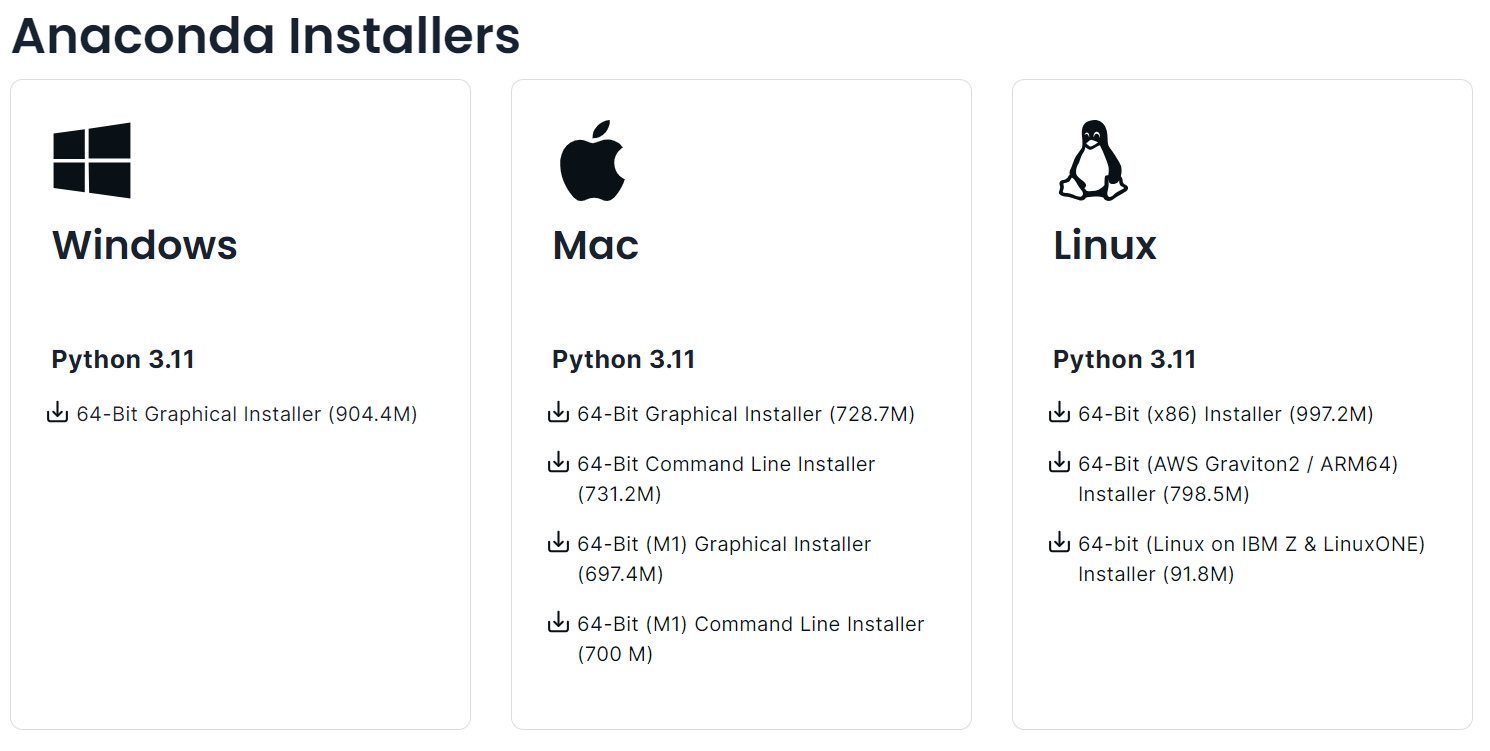
\includegraphics[width=0.99\textwidth]{img/sistema_operativo_anaconda.PNG}
        \caption{Instalación de anaconda según el sistema operativo. Fuente propia.}
        \label{fig:sistema_operativo_anaconda}
    \end{figure}
    \FloatBarrier
    
    Una vez descargado el instalador, se ejecuta y se siguen los pasos que se indican tales como la ubicación donde se desea guardar la aplicación, si se prefiere instalar solo para un usuario o para todos los que haya en el ordenador, etc. según lo que le interese a cada usuario. 
    
\subsubsection{2. Instalación del cuaderno de jupyter en anaconda}
    
    Al abrir la aplicación de anaconda en el sistema ``Anaconda Navigator'', no suele venir instalado el cuaderno de Jupyter Notebook, el cual se emplea para la realización del código por lo que, para instalarlo, se debe acceder al apartado de ``\textit{Home}'' de ``Anaconda Navigator'' y donde pone Jupyter Notebook se le da a ``install'' (si en lugar de poner ``install'', pone ``launch'' quiere decir que ya está instalado y, por tanto no se debe realizar este paso). La figura \ref{fig:instalacion_jupyterNotebook}, es un ejemplo donde el Jupyter Notebook ya está instado.

    \begin{figure}[ht]
        \centering
        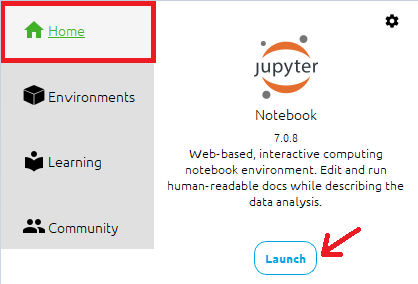
\includegraphics[width=0.70\textwidth]{img/instalacion_jupyterNotebook.PNG}
        \caption{Instalación de Jupyter Notebook realizada correctamente. Fuente propia.}
        \label{fig:instalacion_jupyterNotebook}
    \end{figure}
    \FloatBarrier

\subsubsection{3. Creación de un entorno para trabajar en este proyecto}
    
    La mejor forma de trabajar en Python sin sufrir problemas de versiones y bibliotecas es mediante entornos. Por eso, se emplea anaconda, ya que, permite crear un entorno distinto para cada trabajo que se realiza. De forma que, se pueden instalar diferentes versiones de Python y bibliotecas en los diferentes entornos, asegurando que los proyectos son independientes y no entran en conflicto. 

    Para instalar un nuevo entorno, se debe acceder al apartado ``\textit{Environments}'' de ``Anaconda Navigator'', ``\textit{Create}'', poner el nombre que se desee al entorno de trabajo con el que se va a trabajar y en packages seleccionar Python con la versión deseada tal y como se muestra en la figura \ref{fig:creacion_entorno}.
    
    \begin{figure}[h]
        \centering
        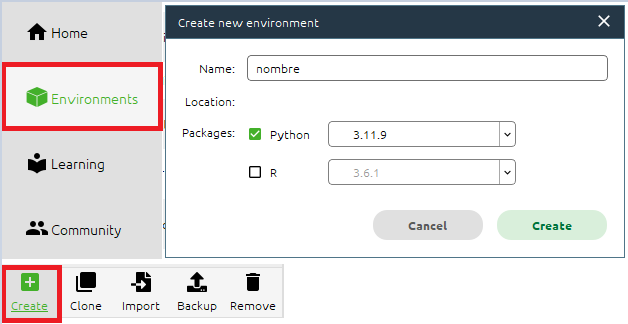
\includegraphics[width=0.99\textwidth]{img/creacion_entorno.PNG}
        \caption{Creación de un nuevo entorno en Anaconda Navigator. Fuente propia.}
        \label{fig:creacion_entorno}
    \end{figure}
    \FloatBarrier
    
    Pero, en este caso, al realizarlo de esta forma surgieron algunos problemas al instalar el paquete Tensorflow, imprescindible para este trabajo, por lo que, tras investigar en la página oficial de anaconda se decidió crear el entorno de una manera distinta. 
    
    Tal y como se indica en la página oficial de anaconda \footnote{\url{https://docs.anaconda.com/free/working-with-conda/applications/tensorflow/}}, una forma de crear un entorno con los paquetes de tensorflow instalados automáticamente es desde la consola de anaconda ``Anaconda Prompt'' a la cual se puede acceder desde el buscador de aplicaciones del sistema tal y como se muestra en la figura (Figura \ref{fig:acceso_consolaAnaconda}).
    
    \begin{figure}[h]
        \centering
        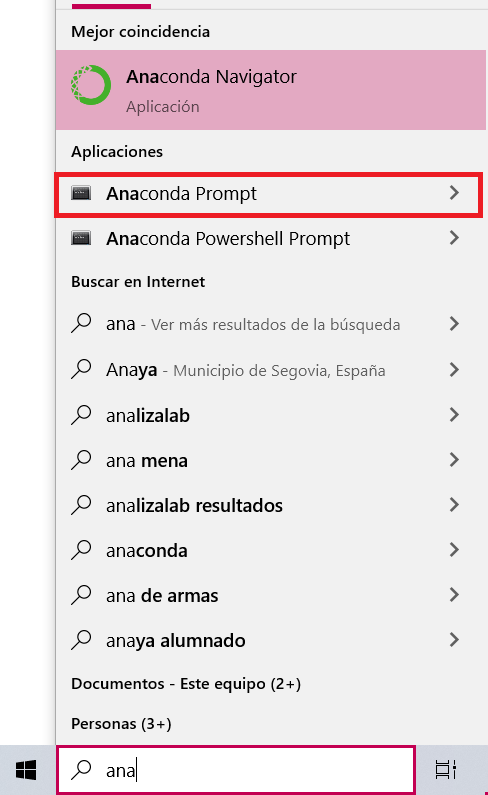
\includegraphics[width=0.60\textwidth]{img/acceso_consolaAnaconda.png}
        \caption{Acceso a la consola de ``Anaconda Prompt''. Fuente propia.}
        \label{fig:acceso_consolaAnaconda}
    \end{figure}
    \FloatBarrier
    
    En la consola de anaconda se debe escribir lo siguiente: ``\textit{conda create -n nombreEntorno tensorflow}'' para crear el entorno con los paquetes necesarios de Tensorflow instalados (Figura \ref{fig:nuevo_entorno}).
    
    \begin{figure}[h]
        \centering
        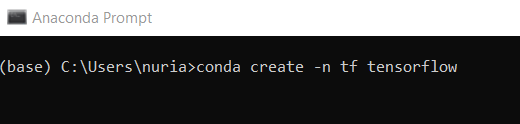
\includegraphics[width=0.99\textwidth]{img/nuevo_entorno.PNG}
        \caption{Creación de un nuevo entorno con Tensorflow con la consola de ``Anaconda Prompt''. Fuente propia.}
        \label{fig:nuevo_entorno}
    \end{figure}
   \FloatBarrier
    
    Una vez creado el entorno, para activarlo, se debe escribir lo siguiente en la consola ``Anaconda Prompt'': ``\textit{conda activate nombreEntorno}''.
    
    A la hora de trabajar con el entorno, se puede acceder tanto al cuaderno de jupyter (``Jupyter Notebook'') como a la consola de ese entorno especifico. Por lo general, se va a acceder al cuaderno de jupyter cada vez que se desee trabajar en el código pero, a la hora de instalar alguna biblioteca nueva o algún paquete necesario se hace a través de la consola (Figura \ref{fig:acceso_entorno}).
    
    \begin{figure}[h]
        \centering
        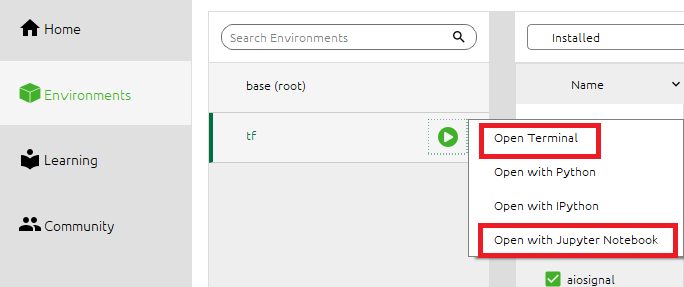
\includegraphics[width=0.99\textwidth]{img/acceso_entorno.png}
        \caption{Acceso a la terminal y Jupyter Notebook del entorno. Fuente propia.}
        \label{fig:acceso_entorno}
    \end{figure}
   \FloatBarrier

    Para instalar los paquetes necesarios bastará con poner en la consola \textit{``conda install nombrePaquete''}. Los paquetes extras que se deben tener instalados para este trabajo además de keras (el cual está dentro de Tensorflow y por lo tanto ya viene instalado con el entorno) son Numpy, Pandas y  Scikit-learn.
    
    Las versiones empleadas en este caso tanto de Python como de tensorflow han sido 3.10.13 y 2.10.0 respectivamente.
    

\section{Instalación / Puesta en marcha}

Una vez se tienen instalados los programas mencionados previamente, ya se puede acceder a los distintos \textit{notebooks} de Python y ejecutar las funciones realizadas para obtener todos los objetivos de este trabajo. Existen tres \textit{notebooks} distintos cuya función se explica a continuación.

\subsection{Carpeta ``data'' y ``data\_nuevo''}

Antes de explicar los distintos \textit{notebooks}, hay que destacar la carpeta ``\textit{data}'', en la cual se encuentran todas las imágenes empleadas para este trabajo y es fundamental para la ejecución de los siguientes \textit{notebooks}.

Dependiendo de donde se encuentre ubicada esta carpeta en el ordenador personal de cada usuario, se deberá cambiar la ruta asignada. Por ejemplo, en este caso, la carpeta se encuentra en la siguiente ruta: \textit{``C:/Users/nuria/Downloads/TFG''} y, por ende, la ruta nueva donde se creará la nueva carpeta con la nueva distribución de las imágenes (toda la explicación referida a esto se encuentra en el \textit{Anexo D}) será \textit{``C:/Users/nuria/Downloads/TFG/data\_nuevo''} en este caso ya que, en el código realizado se ha estipulado que la nueva carpeta se cree en el mismo directorio donde se encontraba la carpeta inicial.

\subsection{\textit{Notebook} ``redes neuronales - neumonía''}

Este es el \textit{notebook} principal con el que se ha trabajado desde un inicio. Incluye todas las funciones necesarias con su ejecución y su correspondiente explicación además de diversas aclaraciones a lo largo de todo el \textit{notebook}. Es el \textit{notebook} en el que se han basado los resultados explicados en la memoria.

Para ejecutar este \textit{notebook}, se han de seguir los siguientes pasos:

\begin{enumerate}
    \item En primer lugar, se han de ejecutar las funciones \textit{buscar\_imagen} y \textit{redestribucion\_imagenes} para obtener la carpeta \textit{data\_nuevo} a partir de la carpeta \textit{data} y, así poder trabajar con las imágenes correctamente distribuidas en las distintas subcarpetas tal y como se explica en el \textit{Anexo D}. 
    
    Hay que tener en cuenta que, con ejecutar esta función una vez, ya se deja creada la carpeta por lo que, no es necesario volver a ejecutarla en ningún otro momento.

    Tal y como se ha comentado previamente, a la hora de llamar a esta función, es necesario indicar el \textit{directorio\_principal} tal y como se muestra en la figura \ref{fig:llamar_funcion_redistrib_imagenes} y, este parámetro debe de ser modificado para cada usuario según donde se encuentre la carpeta \textit{data}.
    \begin{figure}[h]
        \centering
        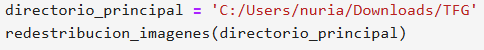
\includegraphics[width=0.99\textwidth]{img/llamar_funcion_redistrib_imagenes.PNG}
        \caption{Llamada a la función \textit{redestribucion\_imagenes} para este caso concreto. Fuente propia.}
        \label{fig:llamar_funcion_redistrib_imagenes}
    \end{figure}
    \FloatBarrier
    
    \item Posteriormente, se debe ejecutar la función \textit{preparar\_modelo} para configurar los generadores de datos para entrenar, validar y probar los modelos.
    \item A continuación, se ejecuta la función \textit{metricas} para calcular las distintas métricas que se van a emplear en la evaluación de los modelos.
    \item Después, se ejecutan las funciones \textit{establecer\_arquitectura\_propia} y \textit{establecer\_arquitectura\_AlexaNet} que establecen los distintos tipos de modelos de red neuronal para para la CNN propia y la de AlexNet que se van a comparar en las siguientes funciones.
    \item Luego, se ejecutan las funciones \textit{arq\_batch\_propia} y \textit{arq\_batch\_AlexNet} con las que se obtiene una tabla comparativa de las métricas calculadas en la función \textit{metricas} para los distintos modelos obtenidos de la función \textit{establecer\_arquitectura\_propia} o \textit{establecer\_arquitectura\_AlexaNet} y distintos valores de \textit{batch size} como son \textit{8, 16, 20, 32 y 64} tanto para la CNN propia como la CNN de AlexNet.

    En la figura \ref{fig:llamada_funcion_arq_batch_propia} se muestra la llamada a la función \textit{arq\_batch\_propia}. El parámetro \textit{ruta}, deberá ser modificado acorde a la ruta donde se encuentre la carpeta \textit{data\_nuevo} según el usuario, tal y como se ha comentado previamente. Los parámetros \textit{nombre\_carpeta\_hist}, \textit{nombre\_carpeta\_resultados} y \textit{nombre\_carpeta\_modelos} se corresponden con los nombres de las carpetas donde se guardan los históricos, los modelos y los resultados finales. En el notebook ``redes neuronales ejecucion archivo.py'' estos nombres son distintos debido a que los resultados que se guardan también lo son tal y como se explica posteriormente. El resto de parámetros son acordes a los modelos, \textit{batch size} y épocas que se han empleado en este trabajo.
    \begin{figure}[h]
        \centering
        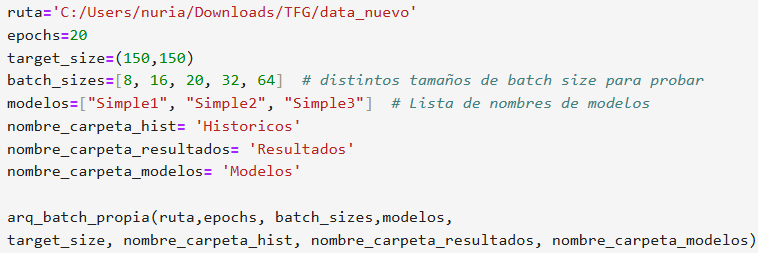
\includegraphics[width=0.99\textwidth]{img/llamada_funcion_arq_batch_propia.PNG}
        \caption{Llamada a la función \textit{arq\_batch\_propia} para este caso concreto. Fuente propia.}
        \label{fig:llamada_funcion_arq_batch_propia}
    \end{figure}
    \FloatBarrier
    \item Una vez se tienen las tablas comparativas de los distintos modelos y distintos \textit{batch size} tanto para la CNN propia como la CNN de AlexNet, ya se puede decidir qué CNN, modelo y \textit{batch size} consigue los mejores valores de métricas. Una vez escogido, se ejecuta la función \textit{neuronas} para el mejor modelo obtenido previamente (en este caso ha sido CNN AlexNet, modelo Simple3 y \textit{batch size} = 64). Con la función \textit{neuronas}, se obtiene una tabla comparativa de las métricas calculadas en la función \textit{metricas} para distintos valores de neuronas (\textit{512, 1024 y 2048}) en la capa oculta con el mejor modelo. A partir de aquí ya se puede determinar el mejor modelo final.

    La llamada a esta función se hace de manera similar a la figura \ref{fig:llamada_funcion_arq_batch_propia} pero con algunos cambios en los parámetros a tratar ya que, en este caso, no se usa como parámetro de entrada ni una lista de \textit{modelos} ni una lista de \textit{batch\_sizes} sino que, el \textit{batch\_size} es un número fijo el cual corresponde con el mejor modelo obtenido previamente. Además se añade un parámetro nuevo denominado \textit{num\_neuronas} que es una lista con los distintos valores de neuronas a probar en la capa oculta y el \textit{target\_size} en este caso es de (340, 340) ya que se emplea la CNN de AlexNet tal y como se puede apreciar en la figura \ref{fig:llamada_funcion_neuronas}.
    \begin{figure}[h]
        \centering
        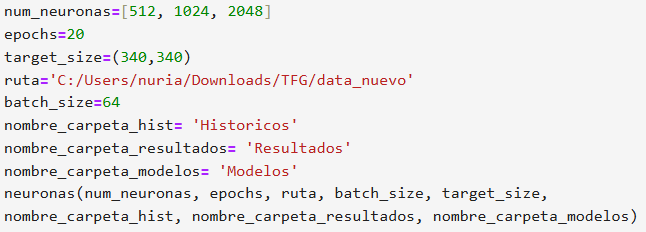
\includegraphics[width=0.99\textwidth]{img/llamada_funcion_neuronas.PNG}
        \caption{Llamada a la función \textit{neuronas} para este caso concreto. Fuente propia.}
        \label{fig:llamada_funcion_neuronas}
    \end{figure}
    \FloatBarrier
    \item Con el mejor modelo de red neuronal ya elegido para este caso, se pueden obtener gráficas para representar la evolución de dos métricas (loss o auc generalmente) durante el entrenamiento y la validación 
    del modelo, lo cual es útil para evaluar el rendimiento del modelo a lo largo de las épocas. Esto se consigue ejecutando la función \textit{grafica} y llamando a dicha función tal y como se muestra en la figura \ref{fig:grafica_auc} donde \textit{directorio\_historico} se refiere a la ruta donde se encuentra el archivo csv con las métricas del modelo del que se desea evaluar el rendimiento (modificar en caso de que la ruta a la carpeta ``Historicos'' sea modificada por el usuario). El parámetro \textit{metrica\_entrenamiento} es la métrica monitoreada durante el entrenamiento que se desea visualizar (en este caso es \textit{auc} aunque podría ser también \textit{loss} para ver el error) y, \textit{metrica\_validacion} se corresponde con la métrica monitoreada durante la validación que se desea visualizar (en este caso es \textit{val\_auc} pero, también podría ser \textit{val\_loss}). 
    \begin{figure}[h]
        \centering
        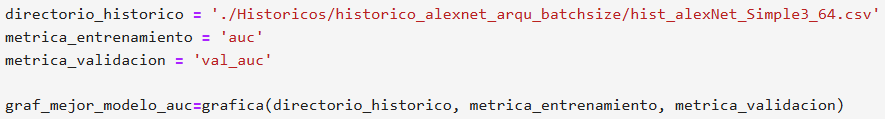
\includegraphics[width=0.99\textwidth]{img/grafica_auc.PNG}
        \caption{Llamada a la función \textit{grafica} con la métrica AUC. Fuente propia.}
        \label{fig:grafica_auc}
    \end{figure}
    \FloatBarrier
    \item Por último, se puede comparar el modelo más simple, (el cual se corresponde con el modelo Simple1 de la CNN propia) con el modelo final elegido por medio de sus matrices de confusión gracias a la función \textit{matriz\_conf}. La figura \ref{fig:llamar_funcion_matriz} muestra un ejemplo de cómo llamar a esta función para obtener la matriz de confusión del modelo más simple. El parámetro inicial \textit{ruta}, se corresponde con el directorio donde se encuentra la nueva carpeta creada con las imágenes \textit{data\_nuevo} y, deberá modificarse acorde a la ruta de esa carpeta para cada usuario. El parámetro \textit{modelo}, se refiere a la ruta donde se encuentra el archivo con el modelo que se desea emplear, en este caso, el modelo obtenido de la CNN propia, Simple1 y un \textit{batch size} de 8 (modificar en caso de que la ruta a la carpeta ``Modelos'' sea modificada por el usuario).
    \begin{figure}[h]
        \centering
        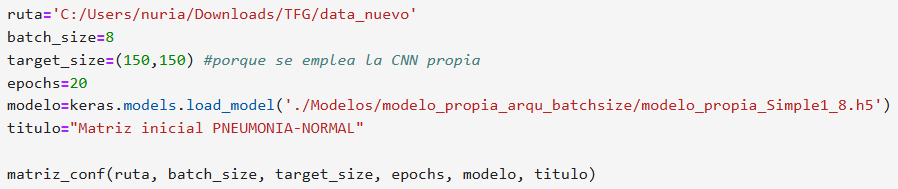
\includegraphics[width=0.99\textwidth]{img/llamar_funcion_matriz.PNG}
        \caption{Llamada a la función \textit{matriz\_conf} para obtener la matriz de confusión inicial. Fuente propia.}
        \label{fig:llamar_funcion_matriz}
    \end{figure}
\end{enumerate}
\FloatBarrier


Algo a tener en cuenta tanto en este \textit{notebook} como en el que se explica a continuación (``redes neuronales ejecucion archivo.py'') es que, en las funciones implementadas ``\textit{arq\_batch\_propia}'', ``\textit{arq\_batch\_AlexNet}'' y ``\textit{neuronas}'', se crean y se guardan dentro de una carpeta denominada ``Historicos'' o ``Historicos\_Py'' (según si se trata del primer \textit{notebook} o del segundo), distintos csv con las métricas obtenidas en el entrenamiento y la validación en cada bucle dependiendo de la función. Por ejemplo, a partir de este \textit{notebook}, en la función ``\textit{arq\_batch\_propia}'' se crea la carpeta ``Historicos'', con distintas subcarpetas, las cuales incluyen distintos ficheros csv para cada modelo y cada \textit{batch size}. A partir de estos csv, se puede crear posteriormente una gráfica para ver el rendimiento del modelo para el entrenamiento y la validación. 

En estas 3 funciones mencionadas previamente, también se crea una carpeta denominada ``Modelos'' con distintas subcarpetas donde se guardan los distintos modelos obtenidos tras el entrenamiento y una carpeta denominada ``Resultados'' con los \textit{dataframes} finales obtenidos para comparar las distintas métricas tras cada función. 

Las carpetas ``Historicos'', ``Modelos'' y ``Resultados'', están configuradas para crearse en el directorio actual, es decir, en la misma ruta en la que se encuentra el \textit{notebook} con el que se está trabajando y, solo en caso de no estar creadas ya. Si, por el contrario, el usuario prefiere guardar dichas carpetas en otro directorio, deberá modificar las tres funciones donde se crean las carpetas tal y como se explica a continuación.

Se va a poner el ejemplo con la función ``\textit{arq\_batch\_propia}'' y la carpeta de ``Historicos'' aunque, se realizaría de igual manera en las otras dos funciones y con las carpetas ``Modelos'' y ``Resultados''. 

En primer lugar, se ha de buscar la línea que pone \textit{ruta\_historicos = os.path.join('.', nombre\_carpeta\_hist)} en la función ``\textit{arq\_batch\_propia}'', donde se crea la ruta a la nueva carpeta de Historicos en el directorio actual. Para modificar esto y que, en lugar de crearse la ruta en el directorio actual se cree en otro directorio, bastará con modificar el punto \textit{'.'} por el directorio que se desee, por ejemplo \textit{``C:/Users/nuria/Downloads/TFG''} o, por el contrario, poner un nombre como puede ser \textit{directorio\_principal}, introducir este parámetro como parámetro inicial de la función y, a la hora de llamar a la función indicar que  \textit{directorio\_principal=``C:/Users/nuria/Downloads/TFG''}, tal y como se muestra en la figura \ref{fig:directorio_modelos_hist_result}. 

Hay que tener en cuenta que, en el caso de modificar alguna ruta, también habrá que modificar las rutas cuando se desea acceder a esas carpetas, por ejemplo, a la hora de llamar a la función \textit{grafica}, el parámetro de entrada \textit{directorio\_historico} tendrá que actualizarse a la nueva ruta y, lo mismo ocurre con la función \textit{matriz\_conf} y el parámetro \textit{modelo}.

\begin{figure}[h]
    \centering
    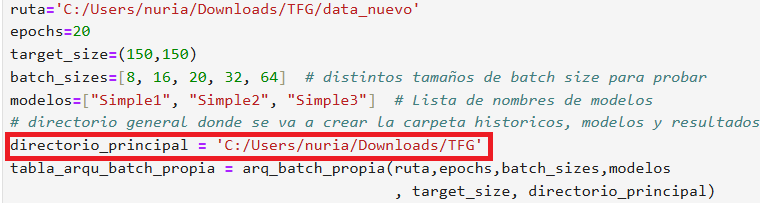
\includegraphics[width=0.99\textwidth]{img/direct_model_hist_result.png}
    \caption{Llamada a la función \textit{arq\_batch\_propia}. Fuente propia.}
    \label{fig:directorio_modelos_hist_result}
\end{figure}
\FloatBarrier


Otro punto a tener en cuenta es que, en este caso los mejores resultados se han obtenido para el modelo ``Simple3'' y, por tanto, la función \textit{neuronas} está configurada para este modelo, sin embargo, debido a la aleatoriedad de pesos y de muestras iniciales y a las similitudes en los resultados obtenidos en el modelo ``Simple2'' y ``Simple3'' explicado en el apartado de ``\textit{Resultados}'' de la memoria, en otra ejecución se puede obtener como mejor modelo el ``Simple2'' y la función \textit{neuronas} ya no serviría para este caso por lo que, a continuación se muestra qué habría que modificar en dicha función para adaptarlo a este modelo.

En la figura \ref{lst:neuronas_simple3} se muestra el fragmento de la función neuronas que deberá ser modificado. En este caso se corresponde con el modelo Simple3. En la figura \ref{lst:neuronas_simple2} se muestra el nuevo fragmento de código (perteneciente al modelo Simple2) que deberá ser sustituido por \ref{lst:neuronas_simple3} en la función \textit{neuronas}.

\begin{lstlisting}[caption={Segmento de la función neuronas correspondiente al modelo Simple3}, label={lst:neuronas_simple3}]
model = keras.Sequential(
            [
                keras.Input(shape=input_shape),
                layers.Conv2D(filters=96, kernel_size=(11,11), strides=(4,4), padding='valid', activation='relu'),
                layers.MaxPooling2D(pool_size=(3,3), strides=(2,2), padding='valid'),
                layers.BatchNormalization(),
                
                layers.Conv2D(filters=256, kernel_size=(5,5), strides=(1,1), padding='valid', activation='relu'),
                layers.MaxPooling2D(pool_size=(3,3), strides=(2,2), padding='valid'),
                layers.BatchNormalization(),
                
                layers.Conv2D(filters=384, kernel_size=(3,3), strides=(1,1), padding='valid', activation='relu'),
                layers.Conv2D(filters=384, kernel_size=(3,3), strides=(1,1), padding='valid', activation='relu'),
                layers.Conv2D(filters=256, kernel_size=(3,3), strides=(1,1), padding='valid', activation='relu'),
                layers.MaxPooling2D(pool_size=(3,3), strides=(2,2), padding='valid'),
                layers.BatchNormalization(),
                
                layers.Flatten(), 
                layers.Dense(neurona, activation='relu'), 
                layers.Dropout(0.2),
                layers.Dense(neurona, activation='relu'), 
                layers.Dropout(0.2),
                layers.Dense(1, activation='sigmoid'), 
            ]
        )
\end{lstlisting}


\begin{lstlisting}[caption={Segmento de la función neuronas correspondiente al modelo Simple2}, label={lst:neuronas_simple2}]
model = keras.Sequential(
            [
                keras.Input(shape=input_shape),
                layers.Conv2D(filters=96, kernel_size=(11,11), strides=(4,4), padding='valid', activation='relu'),
                layers.MaxPooling2D(pool_size=(3,3), strides=(2,2), padding='valid'),
                layers.BatchNormalization(),
                
                layers.Conv2D(filters=256, kernel_size=(5,5), strides=(1,1), padding='valid', activation='relu'),
                layers.MaxPooling2D(pool_size=(3,3), strides=(2,2), padding='valid'),
                layers.BatchNormalization(),
                
                layers.Conv2D(filters=384, kernel_size=(3,3), strides=(1,1), padding='valid', activation='relu'),
                layers.Conv2D(filters=384, kernel_size=(3,3), strides=(1,1), padding='valid', activation='relu'),
                layers.Conv2D(filters=256, kernel_size=(3,3), strides=(1,1), padding='valid', activation='relu'),
                layers.MaxPooling2D(pool_size=(3,3), strides=(2,2), padding='valid'),
                layers.BatchNormalization(),
                
                layers.Flatten(), 
                layers.Dense(neurona, activation='relu'), 
                layers.Dropout(0.2),
                layers.Dense(1, activation='sigmoid'), 
            ]
        )

\end{lstlisting}

\subsection{Archivo ``Funciones.py''} 

Un archivo <<.py>> es un archivo con código fuente de Python que se emplea para guardar scripts u otros archivos de Python. Es de gran utilidad para ejecutar las funciones desde cualquier computador ya que, los archivos <<.py>> pueden ser abiertos y editados desde cualquier editor de texto que contenga el intérprete Python \cite{onlineconvert24}.

Por lo tanto, el archivo ``Funciones.py'' incluye todas las funciones implementadas en el \textit{notebook} ``redes neuronales - neumonía'' para, poder ser ejecutadas desde cualquier editor de texto.

\subsection{\textit{Notebook} ``redes neuronales ejecucion archivo.py''} 

En este \textit{notebook} se muestra cómo importar y utilizar las funciones desde el archivo Funciones.py.

Por lo que se han vuelto a ejecutar todas las funciones del \textit{notebook} ``redes neuronales - neumonía'' pero esta vez, siendo importadas a partir del archivo <<.py>>.

Los resultados de las funciones en estos dos \textit{notebooks} pueden variar sutilmente ya que, como ya se ha comentado en el apartado de ``Resultados'' de la memoria, cada vez que se entrena el modelo, tanto los pesos iniciales como las muestras de entrenamiento se asignan de manera aleatoria por lo que los resultados pueden ser ligeramente distintos. Es por esto que, se han creado carpetas donde guardar los históricos, modelos y resultados específicas para este \textit{notebook} denominadas\textit{ Historicos\_Py}, \textit{Modelos\_Py} y \textit{Resultados\_Py}.


\section{Demostraciones prácticas}

Todas las demostraciones prácticas se encuentran correctamente explicadas y ejecutadas en cada uno de los \textit{notebooks} mencionados previamente.





    
     
\apendice{Manual del programador} % usar el término que mejor se corresponda.

\section{Estructura de directorios}

Todos los directorios mencionados a continuación, se encuentran en el repositorio de GitHub \textbf {TFG-Numonia-RedesNeuronales} \footnote{\url{https://github.com/NuriaMartinez/TFG-Numonia-RedesNeuronales}}, el cual, está compartido con el tribunal de este TFG.
\begin{itemize}
    
    \item \textbf{README.md}: documento escrito en formato \textit {Markdown}, el cual incluye el resumen del trabajo, una pequeña explicación general del contenido del respositorio de GitHub y una breve descripción acerca de los datos empleados para este trabajo, además de los links a \textit{onedrive}  para descargarse las carpetas ``data'' y ``data\_nuevo''. Ya que, al tratarse de una gran cantidad de imágenes es necesario compartirlo de esta forma. Las carpetas se encuentras comprimidas en \textit{zip}, por lo que, una vez descargadas, antes de empezar a trabajar con ellas, es necesario descomprimirlas.
    \begin{itemize}
        \item \textbf{Carpeta ``data''}: carpeta descargada de internet que incluye tres subcarpetas (``\textit{train}'', ``\textit{test}'' y ``val'') y, estas a su vez incluyen dos subcarpetas (``NORMAL'' y ``PNEUMONIA'') con todas las imágenes de CXT con las que se trabaja en este proyecto.
        \item \textbf{Carpeta ``data\_nuevo''}: tal y como se explica en el \textit{Anexo D}, la carpeta ``data'' no contiene una distribución correcta para trabajar con las imágenes por lo que, empleando Python, se ha creado una nueva carpeta denominada ``data\_nuevo'' con las imágenes distribuidas de una forma proporcional para trabajar correctamente con ellas.
    \end{itemize}
    
    \item \textbf{Carpeta ``codigo''}: en esta carpeta se incluyen los dos \textit{notebooks} de Python y el archivo.py donde se ha realizado toda la parte de programación. Para más información consultar el \textit{Anexo B}. Además, también se encuentra la carpeta ``pics'', con las imágenes incluidas a modo decorativo en los distintos \textit{notebooks} y README.md de GitHub y una serie de carpetas obtenidas a partir de la ejecución de los \textit{notebooks}. 
    
    Debido al espacio limitado de GitHub, no es posible incluir directamente en el repositorio las carpetas generadas automáticamente al ejecutar el código. Por lo tanto, se ha creado un archivo README.md con los enlaces a dichas carpetas comprimidas a través de \textit{OneDrive}. Para acceder a su contenido, bastará con descargarlas y descomprimirlas. Las carpetas incluidas en estos enlaces son:
    
    \begin{itemize}
        \item \textbf{Carpeta ``Datos''}: en esta carpeta se incluyen 5 archivos en formato csv, los cuales se corresponden con los distintos \textit{dataframes} obtenidos en la primera función \textit{``redestribucion\_imagenes''}. En la cual, se busca redistribuir las imágenes de la carpeta \textit{data} de una forma más equitativa. Todos los csv están formados por dos columnas ``nombres\_ficheros'' que corresponde con el nombre de las imágenes y ``clases'' que puede ser un 1 o un 0 en función si la imagen tiene neumonía o no. 
        \begin{itemize}
            \item En el csv denominado \textit{\textbf{dataset\_info}} se muestra el nombre de todas las imágenes existentes en la carpeta data con su correspondiente clase (0 o 1). 
            \item El csv \textit{\textbf{test\_dataset\_info}} se corresponde con la proporción de imágenes seleccionadas para \textit{test}, es decir el 20\% del csv \textit{dataset\_info}, existiendo una proporción entre las clases. 
            \item El csv \textit{\textbf{train\_dataset\_info}} se corresponde con el 80\% del csv \textit{dataset\_info} ya que, antes de obtener la proporción de \textit{train} final, se realiza una distribución de 80/20 para \textit{train} y para \textit{test} y, posteriormente, el 80\% de \textit{train} se divide entre \textit{train} y \textit{val} para obtener la proporción final. Por lo que, se podría decir que, este csv forma parte del proceso de la realización de la función \textit{``redestribucion\_imagenes''} pero no se emplea para la redistribución definitiva.
            \item El csv \textit{\textbf{train\_final\_dataset\_info}} es el \textit{dataframe} final de \textit{train}. Se corresponde con una proporción del 64\% del csv \textit{dataset\_info} con una proporción entre las clases.
            \item Por último, el csv \textit{\textbf{val\_dataset\_info}} se corresponde con una proporción del 16\% del csv \textit{dataset\_info}. También existe una proporción entre las clases.
        \end{itemize}
        \item \textbf{Carpeta ``Historicos''}: en esta carpeta se incluyen diversas subcarpetas, cada una de ellas perteneciente a un modelo o \textit{batch size} determinado para CNN propia o CNN Alex Net y para distinto número de neuronas. Dentro de cada subcarpeta, se encuentran distintos csv obtenidos para cada uno de esos casos. En estos csv se incluyen los valores de diferentes métricas obtenidas durante el entrenamiento en cada época para ese modelo, \textit{batch size} o número de neuronas concretos.
        \begin{itemize}
            \item Los csv dentro de la carpeta denominada\\ \textit{\textbf{historico\_propia\_arqu\_batchsize}} se corresponden con las métricas obtenidas para cada época durante el entrenamiento de los modelos Simple1, Simple2 y Simple3 y los valores de \textit{batch size} 8, 16, 20, 32 y 64 con la CNN propia.
            \item Los csv dentro de la carpeta denominada\\ \textit{\textbf{historico\_alexnet\_arqu\_batchsize}} se corresponden con las métricas obtenidas para cada época durante el entrenamiento de los modelos Simple1, Simple2 y Simple3 y los valores de \textit{batch size} 8, 16, 20, 32 y 64 con la CNN de AlexNet.
            \item Los csv dentro de la carpeta denominada\\ \textit{\textbf{historico\_neuronas}} se corresponden con las métricas obtenidas para cada época durante el entrenamiento del modelo Simple3, basado en la CNN de AlexNet y un \textit{batch size} de 64 con distintos números de neuronas en la capa oculta (512, 1024 y 2048). 
            
        \end{itemize}
        Estos csv han sido obtenidos a partir de la ejecución realizada en el \textit{notebook} ``redes neuronales - neumonia''.
        \item \textbf{Carpeta ``Historicos\_Py''}: La explicación para todos los archivos que se encuentran en esta carpeta coincide con la explicación de la carpeta anterior excepto por un detalle. Y es que, todos los archivos de la carpeta ``Historicos\_Py'' se corresponden con la ejecución realizada en el \textit{notebook} ``redes neuronales ejecución archivo.py''. 
        
        La distinción entre estas dos carpetas se debe a que, los resultados de la ejecución en ambos \textit{notebooks} pueden ser sutilmente diferentes debido a la aleatoriedad de pesos y muestras iniciales en cada ejecución (explicado en el apartado de ``\textit{Resultados} de la memoria). Por lo que, los csv almacenados en dichas carpetas también son distintos.
        
        \item \textbf{Carpeta ``Modelos''}: en esta carpeta, al igual que ocurría con la carpeta ``Historicos'', se incluyen diversas subcarpetas, cada una de ellas perteneciente a un modelo o \textit{batch size} determinado para CNN propia o CNN Alex Net y para distinto número de neuronas. Dentro de cada subcarpeta, se encuentran distintos archivos obtenidos para cada modelo y cada \textit{batch size} de la CNN propia, de la CNN Alexnet y para distinto número de neuronas del modelo Simple3 y \textit{bacht size} 64. 

        \begin{itemize}
            \item Los archivos dentro de la carpeta denominada\\ \textit{\textbf{modelo\_propia\_arqu\_batchsize}} se corresponden con los modelos obtenidos durante el entrenamiento de la arquitectura Simple1, Simple2 y Simple3 y los valores de \textit{batch size} 8, 16, 20, 32 y 64 con la CNN propia.
            \item Los archivos dentro de la carpeta denominada\\ \textit{\textbf{modelo\_alexnet\_arqu\_batchsize}} se corresponden con los modelos obtenidos durante el entrenamiento de la arquitectura Simple1, Simple2 y Simple3 y los valores de \textit{batch size} 8, 16, 20, 32 y 64 con la CNN de AlexNet.
            \item Los archivos dentro de la carpeta denominada\\ \textit{\textbf{modelo\_neuronas}} se corresponden con los modelos obtenidos durante el entrenamiento de la arquitectura Simple3, basado en la CNN de AlexNet y un batch size de 64 con distintos números de neuronas en la capa oculta (512, 1024 y 2048). 
            
        \end{itemize}
    
        Estos archivos, se encuentran en un formato HDF, el cual se emplea para almacenar grandes cantidades de datos (numéricos, gráficos y de texto) de una forma jerárquica, por lo que, la gestión de estos datos se realiza de una forma eficiente \cite{filext24}. 
    
        Dentro de cada archivo, se encuentran los valores de pesos del modelo, su estructura completa (capas, conexiones, etc.), información sobre el optimizador y su estado y la configuración de compilación del modelo que incluye la función de pérdida y las métricas \cite{TensorFlowSave24}.
    
        Al igual que ocurría en el caso anterior, en esta carpeta se guardan los archivos referidos al \textit{notebook} ``redes neuronales - neumonia''.
        \item \textbf{Carpeta ``Modelos\_Py''}: con esta carpeta ocurre exactamente lo mismo que con la carpeta ``Historicos\_Py''. Toda la explicación de cada uno de sus archivos coincide con la ya detallada en la carpeta ``Modelos'' pero, con la diferencia de que, los archivos de esta carpeta se obtienen a partir de la ejecución \textit{notebook} ``redes neuronales ejecución archivo.py''. 
    
        \item \textbf{Carpeta ``Resultados''}: en esta carpeta se incluyen los distintos \textit{dataframes} en formato csv donde se muestran las tablas comparativas obtenidas en este trabajo. 
        \begin{itemize}
            \item El archivo \textit{\textbf{compara\_propia\_arqu\_batch\_def.csv}} se corresponde con la tabla final obtenida tras el entrenamiento de la arquitectura Simple1, Simple2 y Simple3 y los valores de \textit{batch size} 8, 16, 20, 32 y 64 con la CNN propia. Se observan los valores de distintas métricas para cada arquitectura y cada valor de \textit{batch size}.
            \item El archivo \textit{\textbf{compara\_alexNet\_arqu\_batch\_def.csv}} se corresponde con la tabla final obtenida tras el entrenamiento de la arquitectura Simple1, Simple2 y Simple3 y los valores de \textit{batch size} 8, 16, 20, 32 y 64 con la CNN AlexNet. Se observan los valores de distintas métricas para cada arquitectura y cada valor de \textit{batch size}.
            \item El archivo \textit{\textbf{compara\_neuronas.csv}} se corresponde con la tabla final obtenida tras el entrenamiento de la arquitectura Simple3, basado en la CNN de AlexNet y un batch size de 64 con distintos números de neuronas en la capa oculta (512, 1024 y 2048). Se observan los valores de distintas métricas para los diferentes valores de neuronas en la capa oculta.
            
        \end{itemize}

        Los archivos de esta carpeta se corresponden con la ejecución del \textit{notebook} ``redes neuronales - neumonia''.

        \item \textbf{Carpeta ``Resultados\_Py''}: Al igual que ocurre con las  carpetas anteriores, toda la explicación de cada uno de sus archivos coincide con la carpeta ``Resultados'' pero, en este caso, los archivos de esta carpeta se obtienen a partir de la ejecución \textit{notebook} ``redes neuronales ejecución archivo.py''. 
        
    \end{itemize}
    \item \textbf{Carpeta ``Artículos y libros TFG''}: carpeta donde se encuentran los principales artículos y libros con los que se ha documentado este trabajo. 
    \item \textbf{Carpeta ``img''}: carpeta con todas las imágenes incluidas en la memoria y los anexos.
    \item En el repositorio de GitHub también se encuentran los archivos en formato \textit{pdf} tanto de la memoria como de los anexos del trabajo.
    \item \textbf{Carpeta ``tex''}: carpeta que incluye cada uno de los apartados de la memoria y los anexos en formato LaTex.
    \item \textbf{anexos.tex}: documento LaTex que incluye la organización del archivo PDF de los anexos.
    \item \textbf{memoria.tex}: documento LaTex que incluye la organización del archivo PDF de la memoria.
    \item \textbf{bibliografia.bib}: archivo que contiene toda la bibliografía empleada para la redacción de la memoria.
    \item \textbf{bibliografiaAnexos.bib}: archivo que contiene toda la bibliografía empleada para la redacción de los anexos.
    
\end{itemize}


\section{Compilación, instalación y ejecución del proyecto}

Toda la explicación relacionada con la compilación, instalación y ejecución del proyecto está explicada en el \textit{Anexo B}.


\section{Pruebas del sistema}

En este trabajo se han realizado diversas pruebas con distintos modelos de arquitectura, distintos \textit{batch sizes}, y número de neuronas. 

Se han creado tres modelos de arquitectura diferentes dentro de las funciones ``\textit{establecer\_arquitectura\_propia}'' y ``\textit{establecer\_arquitectura\_AlexaNet}'' los cuales están explicados en el apartado de ``\textit{Metodología}'' de la memoria. Para poder emplear cada uno de estos modelos, se ha de pasar como parámetro inicial de la función el nombre del modelo (``Simple1'', ``Simple2'' o ``Simple3'') con el que se desea trabajar. Un ejemplo de esto se puede observar en la figura \ref{fig:ejemplo_simple1_estab_arq_propia} en la cual, se ejecuta la función ``\textit{establecer\_arquitectura\_propia}'' para el modelo ``Simple1'' y se obtiene un objeto de la clase \textit{Sequential} perteneciente al módulo de keras. A partir de este objeto, se puede trabajar con dicho modelo para entrenarlo, evaluarlo, etc.

\begin{figure}[h]
    \centering
    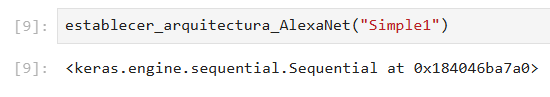
\includegraphics[width=0.99\textwidth]{img/ejemplo_simple1_estab_arq_propia.PNG}
    \caption{Ejecución función \textit{``establecer\_arquitectura\_AlexaNet''} para el modelo Simple1. Fuente propia.}
    \label{fig:ejemplo_simple1_estab_arq_propia}
\end{figure}
\FloatBarrier

En las funciones ``\textit{arq\_batch\_propia}'' y ``\textit{arq\_batch\_AlexNet}'', se comparan los distintos modelos mencionados previamente y distintos valores de \textit{batch size}. Para poder ser comparados los distintos valores de \textit{batch size}, se crea una lista con los valores y se añade como parámetro de entrada de las funciones. En este caso, tal y como se ha podido apreciar en el apartado de ``\textit{Resultados}'' de la memoria, se ha probado una lista de valores de [8, 16, 20, 32, 64]. Para cada modelo y valor de batch size, se obtienen unas métricas de entrenamiento concretas, las cuales se guardan en distintos archivos csv dentro de la carpeta ``Historicos''.

Por último, en la función ``\textit{neuronas}'', se realiza una comparación entre diferentes valores de neuronas para la capa oculta. Al igual que ocurría con el \textit{batch size}, se crea una lista con los distintos valores de neuronas y se añade como parámetro de entrada de la función. Los valores de neuronas a probar en este caso, han sido [512, 1024, 2048] y los resultados obtenidos se pueden ver en el apartado de ``\textit{Resultados}'' de la memoria. Para cada valor de neuronas, se obtienen unas métricas distintas que, también se guardan en la carpeta ``Historicos''.



\section{Instrucciones para la modificación o mejora del proyecto.}

Para que este trabajo pueda ser modificado en futuras ediciones, además de tener en cuenta la estructura del repositorio en GitHub mencionado previamente, se pueden considerar los siguientes puntos:

\begin{itemize}
    \item En este TFG, se han creado tres arquitecturas distintas (Simple1, Simple2 y Simple3) a partir de una CNN propia y de la CNN de AlexNet. En el caso de querer crear nuevas arquitecturas (para probar nuevas capas, nuevos parámetros, etc.), se puede tener en cuenta tanto la función ``\textit{establecer\_arquitectura\_propia}'' como ``\textit{establecer\_arquitectura\_AlexaNet}'' las cuales se encuentras perfectamente documentadas en los \textit{notebooks} de Python. 

    A la hora de modificar estas funciones, una recomendación podría ser mantener las CNN creadas y añadir nuevos modelos (``Simple4'', ``Simple5'', etc) con nuevas capas ocultas, o cambios en los parámetros. O, por el contrario, crear una nueva función con una nueva CNN y nuevos modelos basándose en las funciones ya creadas. 

    Sea como sea, hay que tener en cuenta que, en las siguientes funciones ``\textit{arq\_batch\_AlexNet}'', ``\textit{arq\_batch\_propia}'' y ``\textit{neuronas}'', donde se entrenan y evalúan los diferentes modelos, se emplean las funciones ``\textit{establecer\_arquitectura\_AlexaNet}'' y  ``\textit{establecer\_arquitectura\_propia}'' por lo que, deberán ser modificadas acorde a las nuevas arquitecturas creadas.

    \item Otra mejora, puede ser la implementación de transfer learning. El transfer learning o transferencia de aprendizaje, consiste en la reutilización de la información de un modelo ya pre-entrenado, para la realización de una tarea especifica. Es de gran utilidad en modelos donde no existe una gran cantidad de datos de entrenamiento \cite{diego23}. 

    Algunos modelos que se podrían probar disponibles en keras son: VGG (16, 19), MobileNet (v1, v2), DenseNet (121, 169, 201), entre otros \cite{diego23}. 

    A partir de estos nuevos modelos, se puede comprobar si la red neuronal realizada en este trabajo mejora o no.

    \item Estudiar más a fondo los diferentes parámetros de \textit{EarlyStopping} empleados durante el entrenamiento en las funciones ``\textit{arq\_batch\_AlexNet}'', ``\textit{arq\_batch\_propia}'' y ``\textit{neuronas}'' y probar parámetros nuevos. 

    \item Tal y como se ha comentado en el apartado de ``Líneas futuras'' de la memoria, otra mejora interesante para futuros desarrollos es el aumento de datos, es decir, incorporar nuevas imágenes en el desarrollo de esta red neuronal para mejorar el entrenamiento. 

    Las nuevas imágenes a introducir pueden ser, siguiendo la línea de este TFG, imágenes de CXT frontales de pacientes entre 1 y 5 años o, haciendo referencia a las ``lineas futuras'' y, para mejorar aún más el rendimiento del modelo, introducir imágenes de todos los rangos de edad y de otras vistas no frontales (como puede ser la oblicua, lateral, etc).
\end{itemize}



\apendice{Descripción de adquisición y tratamiento de datos}


\section{Descripción formal de los datos}

En este trabajo, se han empleado imágenes de radiografía de tórax (CXT por sus siglas en inglés), en un formato \textit{.jpeg} obtenidas a partir de una base de datos pública ~\cite{kaggle24}. En esta base de datos, se encuentra una carpeta principal con diversas subcarpetas donde se alojan las imágenes.

La carpeta principal contiene 3 subcarpetas, la de entrenamiento (\textit{train}), validación (val) y prueba (test). Dentro de cada una de estas carpetas hay dos subcarpetas, ``NORMAL'', con las imágenes sin neumonía y ``PNEUMONIA'' con las imágenes de CXT que presentan neumonía.

A su vez, las carpetas de ``PNEUMONIA'' tienen indicado en el nombre del archivo (la imagen) si se trata de una neumonía viral o bacteriana. 

\begin{itemize}
    \item Las imágenes de entrenamiento o \textit{train} se emplean para entrenar el modelo de aprendizaje automático ~\cite{linkdif24}. Dentro de la carpeta ``\textit{train}'', ``NORMAL'' hay un total de 1341 imágenes, y en ``\textit{train}'', ``PNEUMONIA'' hay 3875 imágenes.
    \item Las imágenes de prueba o \textit{test} se emplean para evaluar el rendimiento del modelo después del proceso de entrenamiento y validación. Proporciona una escena objetiva de la precisión del modelo para generalizar datos nuevos ~\cite{linkdif24}. Dentro de la carpeta ``\textit{test}'', ``NORMAL'' hay un total de 234 imágenes, y en ``\textit{test}'', ``PNEUMONIA'' hay 390 imágenes.
    \item Las imágenes de validación o val son una carpeta adicional que ayuda a seleccionar el mejor modelo y evitar el sobreajuste ~\cite{linkdif24}. Dentro de la carpeta ``val'', ``NORMAL'' hay un total de 8 imágenes, y en ``val'', ``PNEUMONIA'' hay 8 imágenes.
\end{itemize}

Las imágenes estaban distribuidas de manera desigual en las carpetas de entrenamiento (\textit{train}) y validación (val). La carpeta de validación contenía únicamente 16 imágenes, mientras que, la carpeta de entrenamiento contenía 5216 imágenes. Esta distribución desbalanceada puede afectar negativamente a la calidad del entrenamiento y la validación del modelo de IA, ya que, una muestra de validación tan pequeña no es representativa y no proporciona una evaluación precisa del rendimiento del modelo. De forma que, se ha creado una nueva distribución de las imágenes.
En la nueva distribución, un 64\% de las imágenes han sido destinadas a \textit{train}, un 20\% para \textit{test} y un 16\% para val. De la misma manera, las imágenes han sido redistribuidas de manera proporcional en cada una de las subcarpetas ``NORMAL'' y ``PNEUMONIA''.

Cada imagen posee un valor distinto de pixeles, es por ello que, antes de comenzar a trabajar con ellas, se realiza un preprocesamiento de imágenes para asociarles a todas ellas el mismo número de pixeles. En este preprocesamiento, también se realiza una normalización de los datos al reescalar los pixeles, de forma que pasan de estar entre un valor de 1 y 255 a estar entre los valores 0 y 1 para poder trabajar correctamente con ellas.

    
\section{Descripción clínica de los datos.}

\subsection{Cosas a tener en cuenta para la realización de una radiografía de rayos X}

Antes meterse en profundidad con las imágenes de radiografía de tórax (CXT por sus siglas en inglés), se van a mencionar algunos puntos importantes a tener en cuenta antes y durante la realización de una radiografía de rayos X:
\begin{itemize}
    \item Se debe verificar la identidad del paciente antes de la realización de la prueba ~\cite{gelaw15}.
    \item El objetivo principal es obtener imágenes de buena calidad a la primera para minimizar la exposición a los rayos X, aunque, si esto no es así, deberán ser desechadas y repetir el proceso ~\cite{gelaw15}.
    \item El paciente debe ser informado acerca de la posición que debe tener su cuerpo y la respiración (inspiración y expiración) que debe realizar ~\cite{gelaw15}.
    \item Se tiene que dar al paciente la bata para ponerse y se deben evitar objetos metálicos alrededor del pecho y cuello (pendientes, collares, etc.) ~\cite{gelaw15}.
    \item Los pacientes con discapacidad tienen preferencia y, en el caso de pacientes con problemas de audición, la explicación tiene que realizarse de forma simbólica o con ayuda del acompañante ~\cite{gelaw15}.
    \item En ocasiones, puede ser necesaria la realización de radiografías desde otras vistas (lateral, oblicua, etc.) para una mejor visualización ~\cite{gelaw15}.
    \item Se debe proteger tanto al personal como al paciente y los acompañantes de la exposición a rayos X. Por ello, se deben aplicar ciertas medidas: emplear una radiación lo más baja posible, proporcionar un delantal de plomo a todos los solicitantes con una protección extra para mujeres embarazadas, las puertas de rayos X deben estar cerrades durante la exposición a la radiación, el personal debe permanecer en una sala protegida durante la exposición y se les debe realizar mediciones periódicas para controlar la radiación, se debe asegurar que la radiación no salga de las salas de rayos X y, por último, las salas de rayos X deben tener una señal de advertencia ~\cite{gelaw15}. 
    
\end{itemize}

Aunque la vista principal para la realización de una CXT es la proyección postero anterior (PA), donde el paciente se sitúa frente a la placa de imagen, en ocasiones con esta vista no se ve claramente alguna anomalía, por lo que, para confirmar o excluir la sospecha, es necesaria la realización de imágenes desde otras vistas ~\cite{gelaw15}:
\begin{itemize}
    \item \textbf{Vista/posición lateral}: se sitúa el lado de interés cerca del detector durante la exposición de la radiación. La imagen se etiqueta según el lado que se coloque frente al detector, por ejemplo, si es el lado derecho, la imagen quedaría etiquetada como ``lateral derecho'' ~\cite{gelaw15}. Figura \ref{fig:CXR_vista_lateral}.
    
    \begin{figure}[!h]
        \centering
        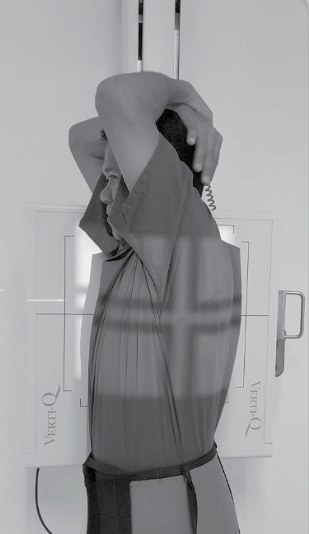
\includegraphics[width=0.30\textwidth]{img/CXR_vista_lateral.PNG}
        \caption{CXT vista lateral. ~\cite{gelaw15}.}
        \label{fig:CXR_vista_lateral}
    \end{figure}
    \FloatBarrier

    \item \textbf{Proyección lordótica}: la parte posterior superior del tórax se sitúa en contacto con el detector. Con esta prueba se consigue que las costillas se alineen longitudinalmente con el haz de rayos X y las clavículas se levanten por encima de los pulmones para poder obtener una vista sin obstáculos de los ápices pulmonares (parte superior del pulmón) y una visualización clara entre las costillas siempre que la técnica y la anatomía lo permitan ~\cite{gelaw15}. Figura \ref{fig:cxr_lordotica}.
    
    Esta vista tiene una variante en la cual el paciente en lugar de tener la parte posterior superior del tórax en contacto con el detector, la parte que tiene en contacto con el detector es la parte anterior inferior del tórax. Es especialmente útil para visualizar los lóbulos inferiores del pulmón desde un ángulo distinto ~\cite{gelaw15}.

    \begin{figure}[h]
        \centering
        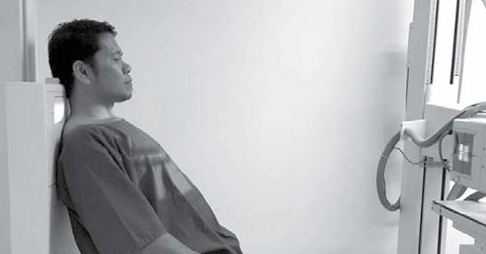
\includegraphics[width=0.55\textwidth]{img/cxr_lordotica.PNG}
        \caption{CXT proyección lordótica. ~\cite{gelaw15}.}
        \label{fig:cxr_lordotica}
    \end{figure}
    \FloatBarrier

    \item \textbf{Posición en decúbito lateral}: el paciente se encuentra tumbado de un lado o del otro y permite determinar la presencia de líquido pleural y neumotórax. Al igual que ocurre con la vista lateral, la imagen se etiqueta según el lado que se coloque frente al detector ~\cite{gelaw15}. Figura \ref{fig:cxr_decubito_lateral}.

    \begin{figure}[h]
        \centering
        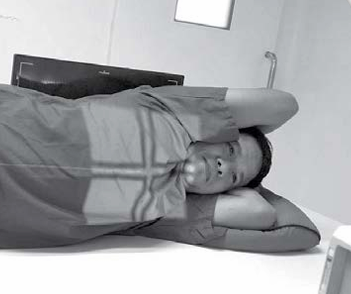
\includegraphics[width=0.50\textwidth]{img/cxr_decubito_lateral.PNG}
        \caption{CXT decúbito lateral. ~\cite{gelaw15}.}
        \label{fig:cxr_decubito_lateral}
    \end{figure}
    \FloatBarrier

    \item \textbf{Vista oblicua}: existen cuatro tipos distintos: oblicua anterior derecha, anterior izquierda, posterior derecha y posterior izquierda. Se puede realizar en posición vertical o tumbado (en caso de que el paciente no pueda mantenerse de pie). Las proyecciones oblicuas anteriores se emplean para la visualización de los pulmones y el mediastino y las vistas oblicuas posteriores se emplean generalmente para la visualización de las costillas y la caja torácica, aunque también pueden realizarse para ver áreas de los pulmones ~\cite{gelaw15}. Se realiza poniendo una de las manos sobre la cabeza tal y como se muestra en la figura \ref{fig:cxr_posterior_oblicua}.

    \begin{figure}[h]
        \centering
        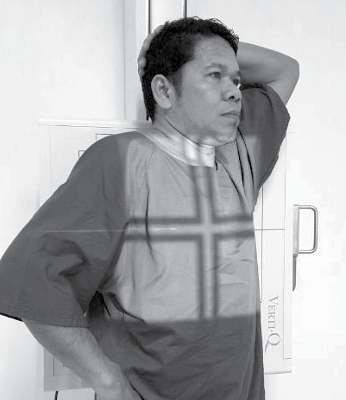
\includegraphics[width=0.40\textwidth]{img/cxr_posterior_oblicua.PNG}
        \caption{CXT posterior oblicua. ~\cite{gelaw15}.}
        \label{fig:cxr_posterior_oblicua}
    \end{figure}
    \FloatBarrier

    \item \textbf{Vista anteroposterior}: se trata de una alternativa a la CXT en posición PA. El paciente se encuentra tumbado con la cara anterior del tórax mirando hacia el detector. Tiene especial interés en personas mayores que no puedes mantenerse de pie o pacientes pediátricos en la misma situación ~\cite{gelaw15}. Por lo tanto, esta CXT puede ser de gran relevancia para este proyecto ya que se trabaja con pacientes de entre 1 y 5 años. Figura \ref{fig:cxr_anteoposterior}.

    \begin{figure}[h]
        \centering
        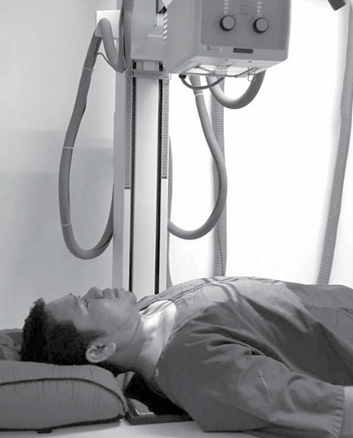
\includegraphics[width=0.40\textwidth]{img/cxr_anteoposterior.PNG}
        \caption{CXT anteoposterior. ~\cite{gelaw15}.}
        \label{fig:cxr_anteoposterior}
    \end{figure}
    \FloatBarrier

    
\end{itemize}

Las radiografías de tórax proporcionan imágenes en blanco y negro donde los huesos se observan de color blanco debido a que bloquean la radiación mientras que los pulmones (al estar llenos de aire) o el aire en sí aparecen como zonas más negras. El corazón también se observa como una zona clara ~\cite{Mayoclinic24}.

Además de contener la imagen correspondiente, las radiografías de tórax también incluyen información biológica relacionada con el paciente para asegurarse que, la imagen pertenece a ese paciente y analizarla correctamente acorde a su edad, sexo, etc. El radiólogo también debe asegurarse de la correcta calidad de la imagen ~\cite{gelaw15}.

\subsection{Análisis de imágenes de CXT}

A la hora de analizar el médico especializado la CXT, lo hace de manera sistemática, es decir, observa de forma ordenada todas las partes de la imagen para detectar posibles anomalías. Una forma de visualizar estas imágenes es comenzar observando las costillas que recubren los pulmones, la columna vertebral, los diafragmas y los recesos costodiafragmáticos. Después, se pasa al corazón y el mediastino y, finalmente a los pulmones. A la hora de ver los pulmones, también se analiza región a región. Este proceso se realiza hasta que todas las zonas de la imágen hayan sido analizadas correctamente ~\cite{gelaw15}.

\begin{itemize}
    \item \textbf{Corazón}: órgano principal del sistema circulatorio que se encarga de bombear sangre a diversos tejidos del cuerpo. Se encuentra en la cavidad torácica, por detrás del esternón y las costillas. El lado derecho del corazón recibe sangre venosa del organismo, es decir, con dióxido de carbono, mientras que, el lado izquierdo del corazón recibe sangre arterial, es decir, sangre oxigenada. Late con una frecuencia de entre 40 y 60 latidos por minuto y tiene un tamaño similar al de un puño ~\cite{CliUniNaCorazon24, CliUniNaSaVenosa24}.
    \item \textbf{Pulmones}: par de órganos ubicados en la cavidad torácica encargados de la función respiratoria y del intercambio de gases entre el aire y la sangre ~\cite{CliUniNaPulmon24}.
    \item \textbf{Costillas}: están constituidas por doce pares de huesos planos, largos y curvos que forma la caja torácica ~\cite{CliUniNaCostilla24}. Su principal función consiste en proteger a los órganos torácicos internos ~\cite{kenhub24}. Otras de sus funciones es la de estructura pasiva en el proceso de la respiración ~\cite{CliUniNaCostilla24}.

    Las costillas se pueden dividir en verdaderas y falsas. Las verdaderas son aquellas que están conectadas directamente con el esternón mientras que las falsas, se conectan al esternón por medio de un cartílago común. Las dos últimas costillas son las también denominadas costillas flotantes ya que, no llegan al esternón ~\cite{CliUniNaCostilla24, kenhub24}. 
    \item \textbf{Columna vertebral}: conjunto de huesos, tendones, músculos y otros tejidos que se extienden desde el cráneo hasta el coxis. Su función consiste en proteger la médula espinal y dar soporte al tronco ~\cite{NIHColVer24, MedliColVer24}
    \item \textbf{Diafragmas}: músculo delgado en forma de cúpula que separa el tórax del abdomen. Se encuentra debajo del corazón y los pulmones. Interviene en el proceso de la respiración ya que, al inhalar se contrae permitiendo que los pulmones se llenen de aire y, al exhalar se relaja permitiendo salir el aire de los pulmones ~\cite{NIHDiaf24, MedliColDiaf24, premiummadridDiaf24}.
    \item \textbf{Recesos costodiafragmáticos}: se trata del espacio entre la pared costal y el diafragma. Interviene en el proceso de la respiración ya que, permite que el diafragma se mueva eficientemente. La presencia de aire, líquido o algún tejido puede indicar la existencia de patologías como cáncer, neumotórax o efusiones pleurales por lo que, es de gran ayuda en el diagnóstico de enfermedades pulmonares ~\cite{CliUniNaReCostodiaf24}.
    \item \textbf{Mediastino}: área anatómica entre los pulmones que engloba órganos como el corazón, los vasos sanguíneos grandes, la tráquea, el timo, el esófago, los bronquios y los ganglios linfáticos ~\cite{NIHmediastino24}.
    
\end{itemize}

Además, en una CXT también se examinan cuidadosamente otras áreas ocultas como las clavículas, vías biliares, ganglios paratraqueales y espacio retrocardiaco ~\cite{gelaw15}.

\begin{itemize}
    \item \textbf{Clavícula}: cada uno de los dos huesos alargados situados en la parte superior del pecho. 
    
    Se articula por su extremo distal con la escápula y por el proximal con el esternón ~\cite{CliUniNaClavicula24, RealAcaEsClavicula24}.
    \item \textbf{Vías biliares}: conductos que conectan el hígado, el intestino delgado y la vesícula biliar de forma que, transportan la bilis desde el hígado hasta el intestino delgado ~\cite{CliUniNabilis24}. 
    
    La bilis es una sustancia generada por el hígado y almacenada en la vesícula biliar. Desempeña un papel importante en la digestión, absorción de las grasas y eliminación de deshechos ~\cite{CliUniNabilis24}.
    \item \textbf{Ganglios paratraqueales}: nodos linfáticos ubicados en la tráquea. Su principal función consiste en combatir las infecciones capturando virus, bacterias y otros agentes patógenos ~\cite{MaCliGanLin24, imaiosGanLin24}.
    \item \textbf{Espacio retrocardiaco}: se trata de un espacio ubicado en el mediastino que queda oculto por el corazón en una CXT frontal permitiendo ver una patología en esa zona cuando aumenta su densidad. Por lo tanto, se convierte en un espacio fundamental para identificar en una radiografía lateral de tórax una posible anomalía en la zona del mediastino ~\cite{canals2022espacio}.
\end{itemize}

A la hora de analizar una imagen de CXT con anomalías evidentes, es importante no dejar pasar otras anomalías más sutiles ~\cite{gelaw15}.

Las anomalías tienen que describirse de la forma más completa posible, esto incluye tipo, ubicación, tamaño, densidad u homogeneidad entre otras ~\cite{gelaw15}.

En imágenes de CXT con una anomalía se pueden distinguir tres tipos: 

\begin{enumerate}
    \item Cambio en la apariencia de la estructura
    \item Área anormalmente blanca (cuando debería ser oscura)
    \item Área anormalmente oscura (cuando debería ser blanca)
\end{enumerate}

En el caso concreto de la neumonía, estaríamos hablando del segundo tipo de anomalía ``área anormalmente blanca'' ya que, los pulmones al absorber poca radiación deberían verse de color oscuro pero, al existir neumonía, se aprecian opacidades blancas en el pulmón denominadas infiltrados pulmonares ~\cite{gelaw15}. 

Los \textbf{infiltrados pulmonares} son alteraciones en los pulmones que se observan como opacidades mal definidas en imágenes como radiografías de tórax. Estas opacidades son cambios en el tejido pulmonar que indican una enfermedad o secuela de una enfermedad pulmonar. Sus causas pueden ser infecciosas, oncológicas, etc  ~\cite{Doctoralia24}. Los infiltrados pulmonares u opacidades blancas se encuentran perfectamente explicados en el apartado de ``Conceptos teóricos'' de la memoria.




\apendice{Especificación de Requisitos}

\section{Diagrama de casos de uso}

Figura \ref{fig:diagrama_casos_uso}.

\begin{figure}[h]
    \centering
    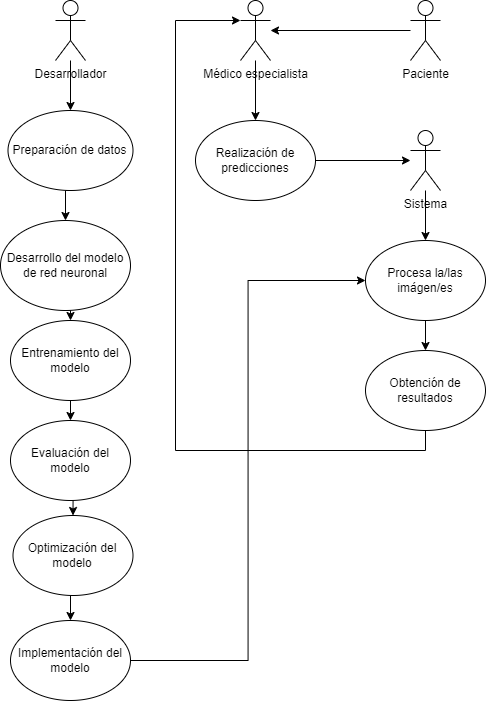
\includegraphics[width=0.99\textwidth]{img/diagrama_casos_uso.PNG}
    \caption{Diagrama de casos de uso realizado con draw.io. Fuente propia.}
    \label{fig:diagrama_casos_uso}
\end{figure}
\FloatBarrier

\section{Explicación casos de uso.}

En este trabajo se ha desarrollado un diagrama de casos de uso \ref{fig:diagrama_casos_uso} que incluye como actores al desarrollador o programador, el neumólogo especializado, el paciente y el sistema. Aunque el enfoque principal de este trabajo ha sido el desarrollo del modelo de red neuronal por parte del desarrollador, se han incluido los casos de uso de los otros actores para ilustrar el potencial y las aplicaciones futuras del proyecto en el ámbito médico.

\subsection{Desarrollador}
El desarrollador es la persona que desarrolla y ajusta el modelo de red neuronal. Sus casos de uso son los siguientes:
\begin{itemize}
    \item \textbf{Preparación de los datos} que incluye tanto la recopilación de imágenes de CXT con y sin neumonía como el preprocesamiento de las imágenes.
    \item \textbf{Desarrollo del modelo de red neuronal} se refiere tanto al desarrollo de la arquitectura de la red neuronal inicial como a los hiperparámetros empleados inicialmente.
    \item \textbf{Entrenamiento del modelo} a partir de las imágenes etiquetadas y su correspondiente validación. También se realiza el ajuste de hiperparámetros según los resultados de validación.
    \item \textbf{Evaluación del rendimiento del modelo} a partir del conjunto de prueba (o test). Para la evaluación del modelo se emplean una serie de métricas como \textit{accuracy}, \textit{recall}, \textit{precision}, AUC, etc.
    \item \textbf{Optimización del modelo} a partir del ajuste de distintos hiperparámetros y reentrenamiento del modelo hasta obtener el idóneo.
    \item \textbf{Implementación del modelo} en un ambiente operativo
\end{itemize}

\subsection{Médico especialista, paciente y sistema}
Como ya se ha comentado en el apartado de ``Líneas futuras'' de la memoria, el objetivo tanto de este trabajo como de otros similares ya realizados es su introducción en el ámbito clínico, aunque, para eso aún son necesarias algunas mejoras. 

Aun así, se ha diseñado también la parte de diagrama de casos de uso llevado al ámbito clínico el cuál se explica a continuación:

\begin{enumerate}
    \item El paciente acude a la consulta con el neumólogo
    \item El médico especializado le realiza una CXT 
    \item Esta imagen es introducida en el sistema previamente desarrollado, el cual es capaz de identificar en esa imagen la presencia o ausencia de neumonía
    \item El sistema muestra en la pantalla del médico si se trata de una neumonía o no
\end{enumerate}




\apendice{Estudio experimental}



\section{Cuaderno de trabajo.}

En esta sección se describen los distintos pasos realizados a lo largo del proyecto con resultados tanto positivos como negativos.

\subsection{Redistribución de las imágenes}

En un principio, se intentó trabajar con las imágenes de CXT descargadas de internet tal y como venían en las carpetas distribuidas en ``\textit{train}'', ``val'' y ``test'' pero, se observó que los resultados que ofrecía no eran buenos, y, esto podía ser debido a una mala distribución en las imágenes. En la carpeta ``val'' venían únicamente 16 imágenes mientras que en la carpeta ``\textit{train}'' había un total de 5216 imágenes, por lo que existía mucho desequilibrio entre el conjunto de imágenes empleadas para el entrenamiento y el conjunto de imágenes empleadas para la validación. Los malos resultados pueden deberse a que una desigualdad entre el conjunto de imágenes de validación y el conjunto de imágenes de entrenamiento está relacionado con el sobreajuste y/o con una mala generalización de datos nuevos.

Por ello, se ha realizado una función en Python a partir de la cual, se distribuye de la manera deseada las imágenes en las distintas carpetas. La manera de distribuirlas ha sido un 64\% de las imágenes han sido destinadas a ``\textit{train}'', un 20\% para ``test'' y un 16\% a ``val''.

\subsection{Preprocesamiento de las imágenes y generación de iteradores}

Una vez obtenida la nueva carpeta con la nueva distribución de imágenes, se realizó otra función para generar iteradores con los conjuntos de entrenamiento, validación y prueba que se emplean para entrenar y evaluar el modelo.

Antes de generar los iteradores se tuvo que realizar un preprocesamiento de las imágenes para poder trabajar correctamente con ellas. Este preprocesamiento incluye un rescaldado de las imágenes, es decir la modificación del valor de los píxeles de [0,255] a [0,1] para normalizar las imágenes y un redimensionamiento de las imágenes a un tamaño de (150,150) o (340,340) según si se emplea la CNN propia o de AlexNet, ya que, las imágenes originales tenían cada una un tamaño distinto, y, para poder trabajar con ellas es necesario que todas tengan el mismo tamaño.

\subsection{Creación del modelo}

El siguiente paso, tras generar los iteradores, consiste en crear el modelo con el que se va a trabajar. Antes de llegar al modelo idóneo se deben probar numerosas combinaciones y numerosos parámetros. En este caso se partió del modelo más simple, compuesto por capas convolucionales, con las que se obtienen características importantes de las imágenes seguidas de capas de MaxPooling2D para reducir la dimensionalidad y sin capas ocultas. A partir de este modelo, se desarrollaron modelos más complejos, con capas ocultas.

A la hora de realizar el modelo más simple (figura \ref{fig:arquitectura_simple}), se probaron distintos valores de ``Dropout'' (0,1; 0,2; 0,3 y 0,5) y se llegó a la conclusión de que los mejores se resultados se obtenían con el 0,2 por lo que es el valor con el que se trabajó a posteriori.

\begin{figure}[h]
    \centering
    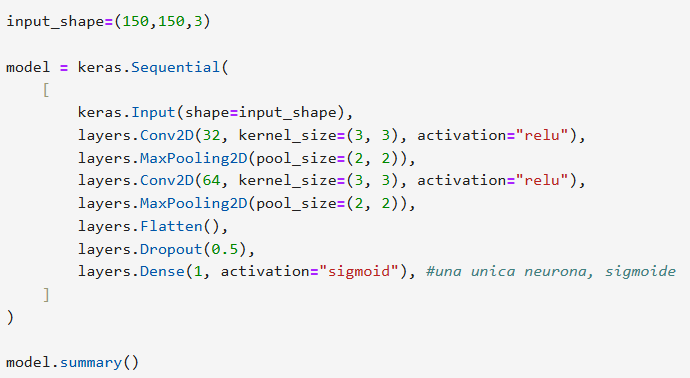
\includegraphics[width=0.99\textwidth]{img/arquitectura_simple.PNG}
    \caption{Modelo de arquitectura más simple. Fuente propia.}
    \label{fig:arquitectura_simple}
\end{figure}
\FloatBarrier

\subsection{Entrenamiento del modelo}

Tras haber creado el modelo, el entrenamiento se produce en dos pasos diferenciados. En primer lugar, se emplea ``model.compile'' para compilar el modelo, y, después ``model.fit'' para entrenarlo.

Al principio, se probó a ejecutar ``model.fit'' sin el parámetro de \textit{EarlyStopping} pero, tras la obtención de malos resultados se recomendó la investigación y el empleo de \textit{EarlyStopping} para una mejora de estos.

\subsection{Evaluación del modelo}

Aunque no se ve reflejado en este trabajo ya que no ha sido empleado finalmente, inicialmente se empleó la función de keras ``model.evaluate'' para la evaluación del modelo y obtención de métricas.

Pero, en este caso, se han calculado las métricas a mano y, se ha obtenido \textit{ytrain} (o las etiquetas de datos de entrenamiento) e \textit{ytest} (o las etiquetas reales de los datos de prueba) para obtener los resultados de las métricas y, a partir de estas métricas evaluar el modelo. Exceptuando la métrica \textit{loss}, la cuál sí se ha calculado a partir de ``\textit{model.evaluate}''.

\subsection{Creación de una función para el cálculo de métricas}

Para la obtención de las diversas métricas, se ha creado una función donde se calculan a mano (a partir de su fórmula) las diversas métricas que se emplean en este trabajo para su evaluación.

Las métricas se calculan a partir de los valores predichos por el modelo (y\_pred) y los valores con las etiquetas reales del conjunto de prueba (y\_test). Una vez se tienen estos dos valores, y, a partir de su matriz de confusión, se obtienen los verdaderos negativos, falsos positivos, falsos negativos y verdaderos positivos y, con esos valores ya se pueden calcular todas las métricas.

\subsection{Realización de diversas funciones para la comparación de diversos modelos, parámetros, etc.}

Una vez realizadas las primeras pruebas y entendidos los diversos pasos a seguir para el entrenamiento y la evaluación de un modelo, se procedió a buscar el mejor modelo para este caso concreto.

Para esto, se comenzó comparando distintos modelos de arquitectura, sin capa oculta, con una capa oculta y con dos capas ocultas. Se creó una función donde se incluyen estos tres modelos de forma que, para compararlos se accede directamente a esta función. 

A continuación, se creó otra función donde se incluye todo lo explicado previamente, es decir, la función donde se crean los iteradores de ``\textit{train}'', ``test'' y ``val'', el modelo con el que se va a trabajar (a partir de la función creada previamente), el entrenamiento del modelo, la evaluación del modelo y la obtención del \textit{dataframe} comparativo de cada modelo con sus correspondientes métricas. El objetivo de esta función fue comprar los distintos modelos y distintos \textit{batch size} para seleccionar el mejor. Para la realización de esta función se tuvieron que realizar algunos cambios en diversos parámetros hasta alcanzar unos resultados aceptables. Por ejemplo, se añadieron y quitaron parámetros de \textit{EarlyStopping}, se cambió la forma de obtención de las métricas en diversas ocasiones, etc.

Tras obtener el mejor modelo y su mejor \textit{batch size}, se creó otra función realizada de forma similar a la anterior para obtener el mejor valor de neuronas en la capa oculta. Al igual que en la anterior función, se llevaron a cabo diversos cambios antes de obtener los parámetros definitivos. En este caso, se tuvieron que probar también múltiples valores de neuronas para la capa o capas ocultas antes de obtener los ideales.

\subsection{Creación de dos CNN, una propia y otra obtenida a partir de la CNN AlexNet}

Debido a que, las métricas obtenidas en un inicio no eran buenas, aunque, los valores obtenidos durante el entrenamiento sí lo eran, además de probar y cambiar varios parámetros hasta encontrar el error, también se realizó un nuevo modelo de CNN, basado en la CNN de AlexNet.

En un principio, esta CNN era solo para comprobar donde estaba el error, pero, finalmente y, tras solucionar el problema de los malos resultados obtenidos en las métricas, se decidió mantener esta CNN para compararla con la CNN creada inicialmente y quedarse con aquella con la que se obtuvieran mejores resultados.

Por lo tanto, a la hora de comparar la mejor arquitectura y el mejor \textit{batch size}, se hizo tanto para la CNN propia como para la CNN basada en AlexNet.


\subsection{Obtención del \textit{dataframe} con las distintas métricas para cada modelo}

El objetivo de todo este proceso consiste en la obtención de un \textit{dataframe} donde se puedan ver y comparar las diversas métricas obtenidas para distintos modelos de red neuronal (con distinta CNN, arquitectura, parámetros, etc.).

Para la obtención de estos \textit{dataframes}, surgieron algunos problemas iniciales ya que, en un principio se imprimía el \textit{dataframe} original, pero, se llegó a la conclusión de que su tamaño era demasiado grande y no se podía mostrar bien en la \textit{memoria} por lo que, se decidió realizar algunos cambios tales como el redondeo a dos decimales de los números, la eliminación del índice o quitar los decimales de números enteros.

Inicialmente tampoco se guardaban estos \textit{dataframes} en ningún sitio, únicamente se imprimían por pantalla en el notebook correspondiente pero, esto se modificó para ser guaradados en formato csv dentro de la carpeta ``Resultados''.

\subsection{Matriz de confusión para la comparación de modelos}

También se ha una función para la obtención de la matriz de confusión del modelo más simple y del modelo final obtenido.

De esta forma se puede comprobar de una forma más visual la mejora de uno respecto al otro.

Para la realización de dichas matrices, es necesario guardar previamente los modelos creados tras cada entrenamiento en las diferentes funciones. De forma que, cuando se desee realizar la matriz de confusión para un modelo en concreto, bastará con cargar dicho modelo. Aunque, cabe mencionar que, inicialmente esto no se hizo así. Al principio, se copiaba y pegaba el modelo para el que se iba a realizar su matriz de confusión y se entrenaba de nuevo. Pero, se comprobó que de esta forma la matriz de confusión obtenida no estaba asociada al 100\% con los resultados de ese modelo obtenidos previamente ya que, debido a la aleatorización explicada en el apartado de \textit{Resultados} de la memoria, cada vez que se entrena el modelo, este puede variar sutilmente. Por lo que, se decidió modificar el código realizado y guardar todos los modelos entrenados para poder ser reutilizados posteriormente dentro de la carpeta ``Modelos''.

\subsection{Gráfica para ver el rendimiento del modelo en el entrenamiento y la validación}

En la creación de las funciones para la obtención de tablas comparativas con diferentes parámetros o arquitecturas, se guardan en un csv los resultados (o métricas) obtenidos en cada iteración para el entrenamiento y la validación dentro de la carpeta ``Historicos''. 

Posteriormente se crea una función para la obtención de una gráfica donde se visualiza el rendimiento del modelo a lo largo de las épocas con la métrica ``\textit{loss}'' o ``auc'' tanto para el entrenamiento como para la validación.

Gracias a esto, se puede observar de una forma más visual si los datos están entrenando correctamente, si existe algún tipo de sobreajuste, subajuste, etc.

\subsection{Se añaden todas las funciones en un archivo.py para ser ejecutadas en otro \textit{notebook}}

Una vez creadas todas funciones necesarias para la realización de este trabajo, se han copiado en un archivo.py para, posteriormente ser ejecutadas en un nuevo \textit{notebook}.

\section{Configuración y parametrización de las técnicas.}

Algunos de los parámetros, hiperparámetros y funciones o clases con una mayor relevancia en este trabajo son:

\begin{itemize}
    \item \textbf{\textit{batch size}}: el tamaño de lote o \textit{batch size}, se explica de forma más extensa en el apartado de ``\textit{Conceptos teóricos}'' de la memoria pero, resumiendo, corresponde con el número de muestras de entrenamiento que se propagarán a través de la red ~\cite{stackbatch24}.
    \item \textbf{\textit{epochs}}: el número de épocas corresponde con las iteraciones que se realizan sobre el conjunto de datos con un determinado \textit{batch size} ~\cite{diego23}. En este caso, se ha empleado un valor de 20 ya que, se trabaja a nivel de CPU (con el ordenador personal) y no GPU (con un supercomputador). Aumentar el número de épocas requeriría más recursos computacionales y tiempo de procesamiento, lo que podría afectar negativamente al rendimiento del ordenador y ralentizar significativamente el proceso de entrenamiento.
    \item \textbf{\textit{class\_mode}}: empleado a la hora de crear cada uno de los iteradores para el entrenamiento y la evaluación del modelo. En este caso se ha empleado el modo 'binary' ya que se trata de una clasificación binaria al haber solo dos clases ``NORMAL'' y ``PNEUMONIA''.
    \item \textbf{\textit{filters}}: se emplea en la clase Conv2D. Es un número entero que determina el número de filtros que tendrá la capa. Generalmente el valor aumenta capa tras capa \cite{kerasconv2d24, diego23}.
    \item \textbf{\textit{kernel\_size}}: se emplea en la clase Conv2D. Número entero o tupla de dos que determina el tamaño de la ventana de convolución o filtro \cite{kerasconv2d24}.
    \item \textbf{\textit{strides}}: se explica de forma más extensa en el apartado de ``\textit{Conceptos teóricos}'' de la memoria pero, resumiendo, corresponde con un número entero o tupla de dos que se emplea en la clase Conv2D y determina el número de columnas y de filas que se desplaza el kernal en cada operación de la convolución\\ \cite{kerasconv2d24, diego23}.
    \item \textbf{\textit{padding}}: se explica de forma más extensa en el apartado de ``\textit{Conceptos teóricos}'' de la memoria, pero, resumiendo, corresponde con un valor tipo \textit{string} que se emplea en la clase Conv2D y afecta a la dimensión de salida de la capa de convolución. Sus dos valores válidos son ``\textit{valid}'' y ``\textit{same}''. Donde ``\textit{valid}'' significa que la dimensión de salida es menor que la de la entrada y ``same'' significa que la longitud de salida es la misma que la longitud de entrada \cite{stackoverflowpadding24}.
    \item \textbf{\textit{pool\_size}}:  Número entero o tupla de dos que se emplea para reducir la dimensionalidad espacial.  En el caso de introducir un número entero, significa que el valor es el mismo para filas y columnas, sin embargo, si se introduce una tupla, el número de filas y columnas puede ser distinto.
    
    Representa el valor máximo de la ventana de entrada sobre el que se va a aplicar MaxPooling2D para realizar un submuestreo de los datos y quedarse con aquellas características más importantes reduciendo la carga computacional y evitando un posible sobreajuste \cite{kerasMaxPool24, diego23}. 
    \item \textbf{\textit{activation}}: a la hora de configurar el modelo, para la capa densa se debe configurar el parámetro \textit{activation}=``sigmoid'' debido a que se trata de un modelo de clasificación binaria y la función sigmoidea siempre devuelve un valor entre 0 y 1 ~\cite{kerassigmoid24}. Donde 0 se corresponde con ``NORMAL'' y 1 con ``PNEUMONIA''.
    \item \textbf{\textit{Dropout}}: ayuda a evitar el sobreajuste ~\cite{kerasdropout24}. En este caso, se han probado diversos valores tales como 0,1; 0,2; 0,3 y 0,5 y se ha determinado que los mejores resultados se obtenían con el 0,2 por lo tanto, es el que se ha empleado.
    \item \textbf{\textit{loss}}: se emplea en \textit{model.compile}, permite configurar el constructor según el argumento que se pase ~\cite{keraslosses24}. En este caso, se ha empleado como argumento la clase \textit{BinaryCrossentropy} ya que, se está trabajando con una clasificación binaria. \textit{BinaryCrossentropy} calcula la pérdida de entropía cruzada entre etiquetas verdaderas y etiquetas predichas ~\cite{kerasbinary24}.
    \item \textbf{\textit{optimizer}}: se trata de un argumento necesario para compilar un modelo Keras ~\cite{kerasOptimizers24}. En este caso, se ha empleado el algoritmo ``adam'', el cual adapta la tasa de aprendizaje para cada parámetro utilizando promedios móviles exponenciales de los gradientes y los cuadrados de los gradientes ~\cite{kerasAdán24}. En este caso, debido a que no se ha indicado ningún valor para \textit{learning rate} concreto, se asume que, se está empleando un \textit{learning\_rate}=0.001 que, es su valor por defecto.
    \item \textbf{\textit{EarlyStopping}}: es una clase la cual se explica extensamente en el apartado de ``\textit{Conceptos teóricos}'' de la memoria pero, resumiendo, su objetivo consiste en dejar de entrenar cuando una métrica monitoreada deja de mejorar ~\cite{kerasearly24}. Esta clase, incluye una serie de argumentos de los cuales, algunos se han incluido en este trabajo y se van a ver a continuación.
    \item \textbf{\textit{monitor}}: argumento de \textit{EarlyStopping} que indica la cantidad que se monitorea ~\cite{kerasearly24}. En este caso se ha empleado ``val\_auc'' ya que es una de las métricas más relevantes para este trabajo.
    \item \textbf{\textit{patience}}: argumento de \textit{EarlyStopping} el cual indica después de cuantas épocas se ha de detener el entrenamiento en caso de que no mejore ~\cite{kerasearly24}. En este caso se ha asignado a 10 épocas.
    \item \textbf{\textit{restore\_best\_weights}}: argumento de \textit{EarlyStopping} con el cual el modelo finaliza con los mejores pesos encontrados durante el entrenamiento al haberlo asignado a ``\textit{True}''. En caso de ser asignado a ``\textit{False}'', el modelo finalizaría con los pesos de la última época entrenada antes de la detención ~\cite{kerasearly24}.

    
\end{itemize}





\apendice{Anexo de sostenibilización curricular}

\section{Introducción}

El 25 de septiembre de 2015 se desarrolló un plan de acción por parte de la Asamblea General de Naciones Unidas a favor de erradicar la pobreza, proteger el planeta y asegurar la prosperidad y la paz universal. Este plan consta de 17 Objetivos de Desarrollo Sostenible (ODS) ~\cite{PaMuReEs24} los cuales se pueden observar en la figura \ref{fig:ODS}.

\begin{figure}[h]
    \centering
    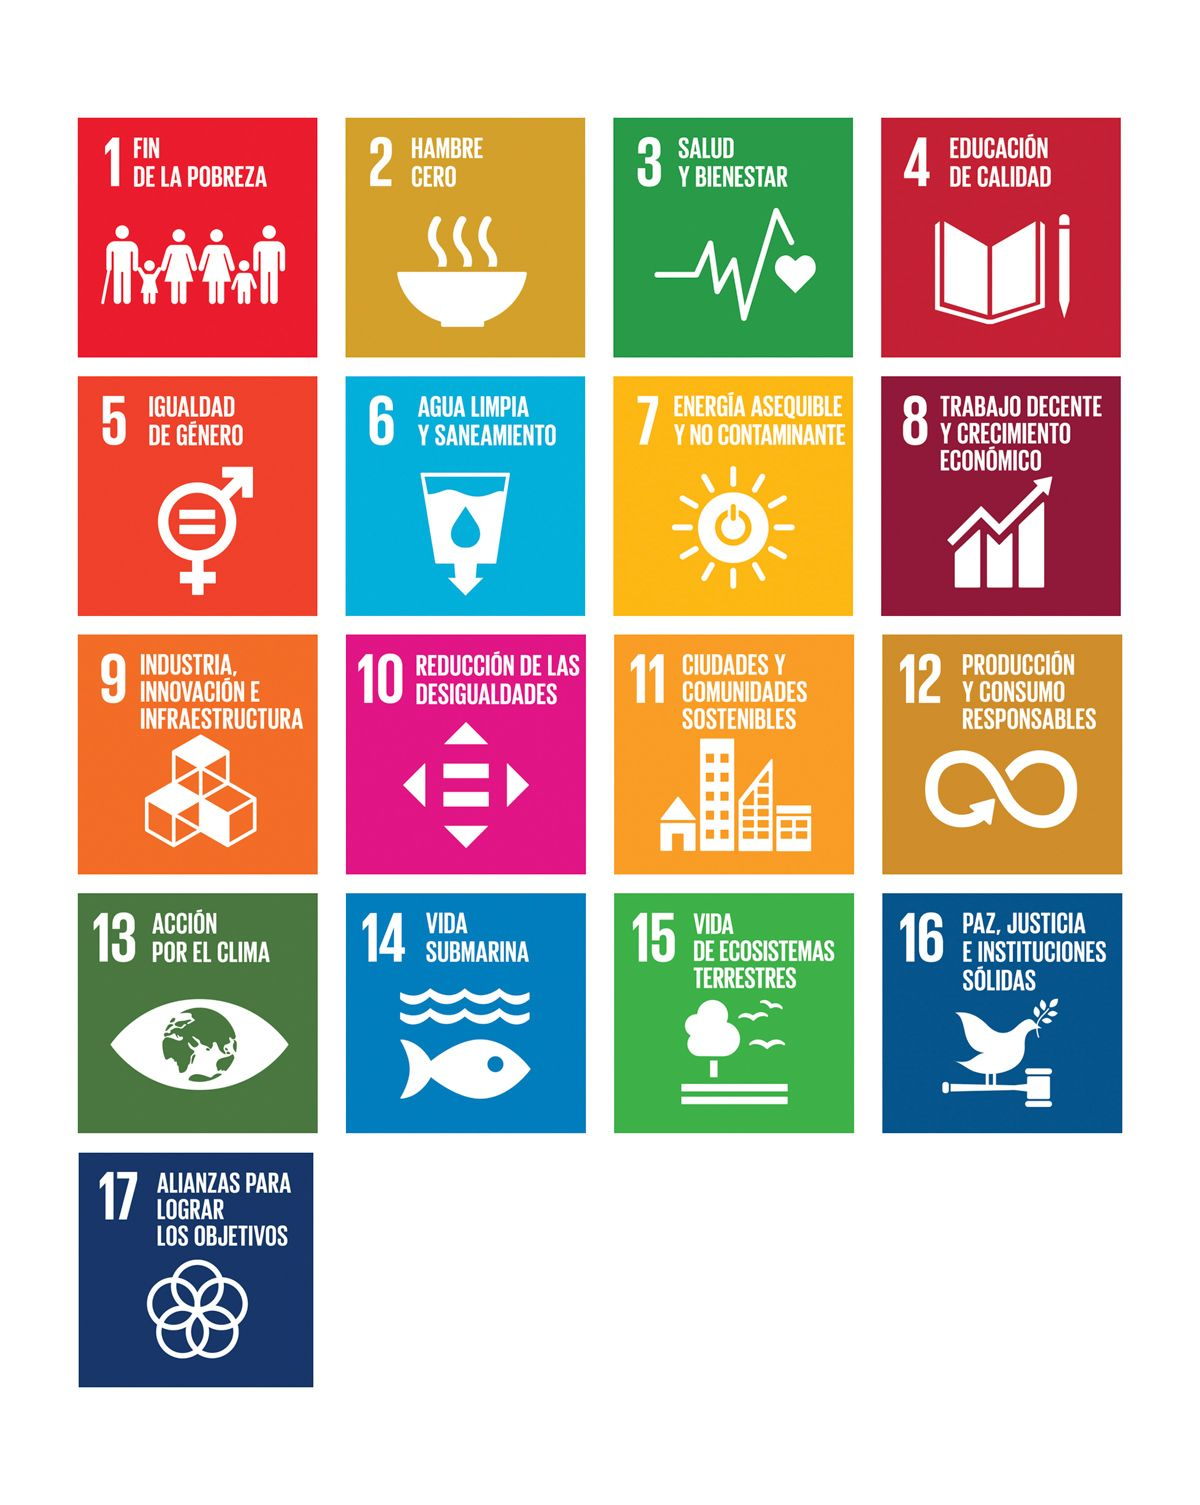
\includegraphics[width=0.99\textwidth]{img/ODS.jpg}
    \caption{ODS Objetivos de Desarrollo Sostenible.~\cite{openbank24} }
    \label{fig:ODS}
\end{figure}
\FloatBarrier

Como ya se ha comentado en otros apartados, el principal objetivo de este trabajo es la obtención de un diagnóstico más rápido, preciso y eficiente. Al margen de todos los beneficios que se pueden conseguir con esto a nivel humano reduciendo la mortalidad por neumonía y mejorando la calidad de vida de los pacientes, también se pueden obtener beneficios a nivel de sostenibilidad y medio ambiente. Ya que, con diagnósticos precisos desde un inicio, se reduce la necesidad de realizar pruebas adicionales para confirmar el diagnóstico, ahorrando tiempo y recursos. Además, también se busca reducir la desigualdad en el acceso a atención médica de calidad a nivel mundial proporcionando una herramienta accesible y eficiente, mejorando así los resultados de salud y promoviendo la equidad global en la atención médica.

Por lo tanto, este trabajo se puede relacionar principalmente con dos de los ODS.

En primer lugar, el\textbf{ ODS 3: ``Salud y bienestar''}, el cual, busca garantizar una vida sana y promover el bienestar para todos en todas las edades ~\cite{ObDeSoSalud24}. Algunas de sus metas son:
\begin{itemize}
    \item \textit{\textbf{ODS 3.2:}  ``Para 2030, \textbf{poner fin a las muertes evitables de recién nacidos y de niños menores de 5 años}, logrando que todos los países intenten reducir la mortalidad neonatal al menos hasta 12 por cada 1.000 nacidos vivos, y la mortalidad de niños menores de 5 años al menos hasta 25 por cada 1.000 nacidos vivos''} ~\cite{ObDeSoSalud24}.

    Tal y como se ha comentado en la memoria, la neumonía es una de las principales causas de muerte en niños menores de cinco años en muchas partes del mundo. Por lo que, con un diagnóstico más preciso y eficiente, se puede ayudar a reducir la mortalidad infantil.
    
    \item \textit{\textbf{ODS 3.3:}  ``Para 2030, poner fin a las epidemias del SIDA, la tuberculosis, la malaria y las enfermedades tropicales desatendidas y combatir la hepatitis, las enfermedades transmitidas por el agua y otras \textbf{enfermedades transmisibles''}} ~\cite{ObDeSoSalud24}. 
    
    La neumonía puede ser una enfermedad muy contagiosa. Por lo que, con un diagnóstico temprano y preciso se puede ayudar a prevenir la propagación y manejar mejor los brotes.

    \item \textit{\textbf{ODS 3.8:}  ``Lograr la \textbf{cobertura sanitaria universal}, en particular la protección contra los riesgos financieros, el \textbf{acceso a servicios de salud esenciales de calidad} y el acceso a medicamentos y vacunas seguros, eficaces, asequibles y de calidad para todos''} ~\cite{ObDeSoSalud24}.

    Este trabajo busca el acceso a una atención médica de calidad a nivel mundial permitiendo que hospitales con recursos limitados puedan acceder a herramientas de diagnóstico avanzadas.

    \item \textit{\textbf{ODS 3.b:}  \textbf{``Apoyar las actividades de investigación y desarrollo de vacunas y medicamentos para las enfermedades transmisibles y no transmisibles} que afectan primordialmente a los países en desarrollo y facilitar el acceso a medicamentos y vacunas esenciales asequibles de conformidad con la Declaración de Doha relativa al Acuerdo sobre los ADPIC y la Salud Pública, en la que se afirma el derecho de los países en desarrollo a utilizar al máximo las disposiciones del Acuerdo sobre los Aspectos de los Derechos de Propiedad Intelectual Relacionados con el Comercio en lo relativo a la flexibilidad para proteger la salud pública y, en particular, proporcionar acceso a los medicamentos para todos''} ~\cite{ObDeSoSalud24}.

    Aunque este trabajo no está directamente enfocado a las vacunas o los medicamentos, sí que fomenta la innovación tecnológica en el diagnóstico médico, lo que promueve grandes beneficios en el ámbito de la salud pública.

    \item \textit{\textbf{ODS 3.d:}  ``Reforzar la capacidad de todos los países, en particular los países en desarrollo, en materia de alerta temprana, reducción de riesgos y \textbf{gestión de los riesgos para la salud nacional y mundial}''} ~\cite{ObDeSoSalud24}.

    Este trabajo busca un rápido diagnóstico de la neumonía, lo que ayuda a reducir riesgos de salud derivados de un mal diagnóstico o un diagnóstico tardío a nivel mundial. 
\end{itemize}

En segundo lugar, este trabajo se puede relacionar con el \textbf{ODS 9: ``Industria, innovación e infraestructuras''} cuyo objetivo consiste en construir infraestructuras resilientes, promover la industrialización sostenible y fomentar la innovación ~\cite{ObDeSoInfraestructura24}. Algunas de sus metas son:
\begin{itemize}
    \item \textit{\textbf{ODS 9.1:} ``Desarrollar infraestructuras fiables, sostenibles, resilientes y de calidad, incluidas infraestructuras regionales y transfronterizas, para apoyar el desarrollo económico y el \textbf{bienestar humano}, haciendo especial hincapié en el acceso asequible y equitativo para todos''} ~\cite{ObDeSoInfraestructura24}.

    La implementación de una red neuronal para el diagnóstico de neumonía promueve el desarrollo de infraestructuras de calidad para apoyar el bienestar humano facilitando el acceso equitativo a los servicios básicos de salud.

    \item \textit{\textbf{ODS 9.2}: ``Promover una industrialización inclusiva y sostenible y, de aquí a 2030, \textbf{aumentar significativamente la contribución de la industria al empleo} y al producto interno bruto, de acuerdo con las circunstancias nacionales, y duplicar esa contribución en los países menos adelantados''} ~\cite{ObDeSoInfraestructura24}.

    Este proyecto contribuye con la modernización e industrialización del sistema sanitario. Lo que genera nuevas oportunidades de empleo en el desarrollo y mantenimiento de sistemas de IA relacionados con la salud.

    \item \textit{\textbf{ODS 9.5:} ``\textbf{Aumentar la investigación científica y mejorar la capacidad tecnológica de los sectores industriales de todos los países}, en particular los países en desarrollo, entre otras cosas fomentando la innovación y aumentando considerablemente, de aquí a 2030, el número de personas que trabajan en investigación y desarrollo por millón de habitantes y los gastos de los sectores público y privado en investigación y desarrollo''} ~\cite{ObDeSoInfraestructura24}.

    Este proyecto, fomenta la innovación tecnológica en el ámbito médico, lo que aumenta la necesidad de contratar profesionales relacionados con la investigación y el desarrollo de la salud digital.

    \item \textit{\textbf{ODS 9.c:} ``\textbf{Aumentar significativamente el acceso a la tecnología de la información} y las comunicaciones y esforzarse por proporcionar acceso universal y asequible a Internet en los países menos adelantados de aquí a 2020''} ~\cite{ObDeSoInfraestructura24}.

    Este trabajo mejora el acceso a tecnologías de la información al facilitar la posibilidad de realizar diagnósticos remotos, de forma que, se puede incrementar la calidad médica en zonas con recursos limitados.
\end{itemize}




\bibliographystyle{apalike}
\bibliography{bibliografiaAnexos}

\end{document}
